%\documentclass[3p,12pt,authoryear]{elsarticle}
\documentclass[3p,12pt]{elsarticle}

\let\counterwithout\relax
\let\counterwithin\relax
%\usepackage{natbib}
%\usepackage{apacite}
\usepackage[colorlinks=true,citecolor=blue,linkcolor=blue]{hyperref}
\usepackage{amsmath,amssymb}
\usepackage{epsfig}  
\usepackage{graphicx}               % Standard graphics package  
\usepackage{url}
\usepackage{titlesec}
\usepackage{hyperref}
\usepackage{cleveref}
\usepackage{color}
\usepackage{listings}

\usepackage{titlesec}

\setcounter{tocdepth}{4}
\setcounter{secnumdepth}{4}

\usepackage{tikz}
\usetikzlibrary{trees}

\tikzstyle{every node}=[draw=black,thick,anchor=west]
\tikzstyle{selected}=[dashed,draw=red,fill=red!30]
\tikzstyle{optional}=[dashed,fill=gray!50]

\usepackage{chngcntr}
\counterwithin{figure}{section}

\titleclass{\subsubsubsection}{straight}[\subsection]
\newcounter{subsubsubsection}[subsubsection]
\renewcommand\thesubsubsubsection{\thesubsubsection.\arabic{subsubsubsection}}
\renewcommand\theparagraph{\thesubsubsubsection.\arabic{paragraph}} % optional; useful if paragraphs are to be numbered

\titleformat{\subsubsubsection}
  {\normalfont\normalsize\itshape}{\thesubsubsubsection}{1em}{}
\titlespacing*{\subsubsubsection}
{0pt}{3.25ex plus 1ex minus .2ex}{1.5ex plus .2ex}

\newcommand{\bra}[1]{\ensuremath{\left\langle#1\right|}}
\newcommand{\ket}[1]{\ensuremath{\left|#1\right\rangle}}
\newcommand{\bracket}[2]{\ensuremath{\left\langle#1 \vphantom{#2}\right| \left. #2 \vphantom{#1}\right\rangle}}
\newcommand{\matrixel}[3]{\ensuremath{\left\langle #1 \vphantom{#2#3} \right| #2 \left| #3 \vphantom{#1#2} \right\rangle}}
\newcommand{\bls}{\begin{lstlisting}}
\newcommand{\els}{\end{lstlisting}}

\newcommand{\ttf}{\ttfamily}
\newcommand{\nuSQUIDS}{{\ttfamily nuSQUIDS}}

\newcommand{\pa}[2]{\frac{\partial #1}{\partial #2}}
\newcommand{\p}[1]{\partial_{#1}}

\newcommand{\jt}[2]{
\item[$\circ$]{#1}
  \begin{lstlisting}
    {#2}
  \end{lstlisting}
}


\definecolor{mauve}{rgb}{1,0,1}
\definecolor{dkgreen}{rgb}{0,0.6,0}
% \definecolor{gray}{rgb}{0.5,0.5,0.5}
% \definecolor{mauve}{rgb}{0.58,0,0.82}

\lstset{language=C++,
%   aboveskip=3mm,
%   belowskip=3mm,
%   showstringspaces=false,
%   columns=flexible,
   basicstyle={\small\ttfamily},
%   numbers=none,
%   numberstyle=\tiny\color{gray},
   morekeywords={SU\_vector,string,Body,Track,marray,Basis},   
   keywordstyle=\color{blue},
   deletekeywords={const},
   keywords=[2]{const},
   keywordstyle={[2]\ttfamily\color{red}},
   deletekeywords={operator},
   keywords=[3]{operator},
   keywordstyle={[3]\ttfamily\color{dkgreen}},
   commentstyle=\color{dkgreen},
   stringstyle=\color{mauve},
%   breaklines=true,
%   breakatwhitespace=true
%   tabsize=3
}

\setcounter{secnumdepth}{4}
\setcounter{tocdepth}{4}

\begin{document}

\begin{frontmatter}

\title{$\nu$-SQuIDS: A toolbox for neutrino oscillations\tnoteref{t1}}

\author[MIT]{Carlos A. Arg\"uelles}
\ead{caad@mit.edu}
\author[UB]{Jordi Salvado}
\ead{jsalvado@icc.ub.edu}
\author[UA]{Christopher N. Weaver}
\ead{chris.weaver@icecube.wisc.edu}
\address[MIT]{Massachusetts Institute of Technology, Cambridge, MA 02139, USA}
\address[UA]{Dept.~of Physics, University of Alberta, Edmonton,
  Alberta, Canada T6G 2E1} 
\address[UB]{Departament de F\'isica Qu\`antica i Astrofísica and Institut de Ciencies del Cosmos,
Universitat de Barcelona, Diagonal 647, E-08028 Barcelona, Spain}

\tnotetext[t1]{The code can be found in \url{https://github.com/arguelles/nuSQuIDS}}
\journal{arXiv}
%\journal{Computer Physics Communications}

\begin{abstract}
The Neutrino Simple Quantum Integro-Differential Solver ($\nu$-SQuIDS)
is a C++ code based on SQuIDS that propagates an ensemble of neutrinos
through a given media. Neutrino oscillation calculations relevant to
current and next generation experiments are implemented. In doing so
we account for coherent and non-coherent neutrino interactions in
different media such as the Sun, Earth, Vacuum, or others.
The code has been design to be accurate and flexible, while at the
same time maintain good performance. It has a modular design that
allows the user to incorporate new physics in novel scenarios. 
\end{abstract}

\begin{keyword}
Neutrino oscillation, phenomenology, collective neutrino behavior, numerical techniques
\end{keyword}

\end{frontmatter}

\hypersetup{linkcolor=black}
\tableofcontents
\hypersetup{linkcolor=blue}
\newpage
\section{Introduction}
\label{sec:intro} 

In recent decades a plethora of evidence that neutrinos change
flavor as they propagate macroscopic distances due to the
non-alignment of their mass and flavor eigenstates has accumulated from
solar~\citep{Abe:2010hy, Borexino2014},
atmospheric~\citep{PhysRevD.91.072004,Richard:2015aua},
accelerator~\citep{PhysRevLett.112.181801,
  PhysRevD.93.051104,PhysRevLett.116.151806, PhysRevLett.110.251801}, and
reactor \citep{An:2013zwz,Abe:2015rcp, Kim:2016yvm} experiments.
Thanks to these remarkable
experimental results and related theoretical calculations the
  neutrino-mass induced flavor oscillation paradigm
\citep{Pontecorvo:1967fh,Gribov:1968kq,fukugita2003physics,
  Akhmedov:1999uz,Balantekin:2013kc, GonzalezGarcia:2007ib,Mohapatra:qv, Gouvea:2013fj}
has been firmly established and the three mixing angles, which
parametrize the lepton mixing matrix, together with the two
squared-mass differences, have been measured to good
precision\citep{Esteban:2016qun,deSalas:2017kay,Capozzi:2018ubv}. It
is the task of on-going 
and future experiments to determine the neutrino mass ordering 
and the CP-violating phase \citep{Hewett:2012et,
  Acciarri:2016crz,Aartsen:2014oha, Kouchner:2016pqa,DeRosa:2016ifc}. 
Also, the IceCube Neutrino Observatory has recently made precise measurements of the atmospheric
spectrum above 100 GeV allowing new physics
models to be constrained~\citep{Aartsen:2014gkd,TheIceCube:2016oqi},
where the Earth is no longer transparent to
neutrinos~\citep{Donini:2018tsg}. 
The identification of high-energy
extraterrestrial neutrinos \citep{ Aartsen:2014gkd, Aartsen:2015rwa}
has opened the possibility of exploring new physics at these energies as well
\citep{Arguelles:2015dca, Bustamante:2015waa, Baerwald:2012kc}. 

Matter effects play a fundamental role in the explanation of solar
neutrinos \citep{ Davis:1968cp,Bethe:1986ej}, which has motivated the study of new flavor
changing neutrino interactions \citep{Barger:1991ae, Roulet:1991sm, GonzalezGarcia:2011my,
  Gonzalez-Garcia:2013usa, Pospelov:2011dp, Kopp:2014nosterile,
  Maltoni:2015kca,Esteban:2018ppq}.
Even though most of the data can be explained in the standard three
neutrino framework, some puzzling anomalies still remain
\citep{LSND,Mention:2011rr,MiniBoone:2012dn,Aguilar-Arevalo:2018gpe,Alekseev:2016llm,
  Ko:2016owz, Ashenfelter:2018iov, Abreu:2018pxg,
  Dentler:2018sju}. These may be explained 
by introducing new light neutrino states \citep{kopp2013sterile,
  Collin:2016rao, Abazajian:2012rf,Blennow:2018hto} and other new physics
\citep{Bai:2015ztj,PalomaresRuiz:2005vf,Gninenko:2011xa}.
Also, the interplay between cosmology and neutrino
oscillation has been widely studied in the literature
\citep{Bergstrom:2014fqa, Giusarma:2016phn,
  Dasgupta:2013la,Hernandez:2016kel,Arguelles:2016uwb,Song:2018zyl,Chu:2018gxk}. 
In counclusion, neutrinos are good proves to perform 
fundamental physics tests~\citep{Hewett:2012et,Aartsen:2017ibm,Mewes:2018cze,Barenboim:2017vlc}.

Tools are needed to accurately and reliably compute neutrino
propagation.
When the only effect of propagation is neutrino oscillations libraries such as {\ttf GLoBES}
\citep{Huber:2007ji}, {\ttf Prob3++} \citep{prob3pp, Calland:2013vaa},
and {\ttf nuCRAFT} \citep{Wallraff:2014vl} are
available. Unfortunately, when non-coherent interactions are 
important they are no longer applicable. Furthermore, the ability to
allow the user to incorporate new physics models or to change the
propagation medium is also limited. {\ttf nuSQuIDS} seeks to
address all of these problems by providing a highly customizable
package, while at the same time remaining numerically efficient.

The rest of the paper is organized as follows: in section
\ref{sec:theory} we review neutrino oscillation theory; in section
\ref{sec:benchmark} we show the use of the code in typical
scenarios; in section \ref{sec:performance} we show the performance of
the library; in section \ref{sec:tests} we describe the unit tests that
are provided with the library; in section \ref{sec:code} we describe
the main classes and structure of the code. Finally, section
\ref{sec:conclu} presents concluding remarks.

\section{Neutrino Oscillations}
\label{sec:theory} 
In this section we briefly review neutrino oscillations
using the density matrix formalism.
We can represent the state of a neutrino ensemble at an energy $E$
and position $x$ using the density matrix. In the weak-interaction flavor-eigenstate basis
$\{\ket{\nu_\alpha}\}$  it can be written as
\begin{equation}
\rho(E,x) = \sum_\alpha \phi_\alpha(E,x) \ket{\nu_\alpha}\bra{\nu_\alpha} , 
\label{eq:state}
\end{equation}
where $\phi_\alpha$ specifies the flux of flavor $\alpha$.
These eigenstates can be related with the mass eigenstates,  $\{ \ket{\nu_i}  \}$, by
\begin{equation}
\ket{\nu_\alpha} = \sum_i U^*_{\alpha i} \ket{\nu_i} ,
\label{eq:changebasis}
\end{equation}
where $U$ is a unitary matrix known as the Pontecorvo-Maki-Nakagawa-Sakata (PMNS)
matrix or neutral lepton mixing matrix. For antineutrinos the relation
is the same as in 
\eqref{eq:changebasis} with $U \to U^*$.
It is customary to parametrize $U$ as a product of complex rotations,
\begin{equation}
\label{eq:mixing}
U(\theta_{ij}\delta_{ij})=R_{N-1\, N} R_{N-2\, N} ... R_{45} R_{35} R_{25} R_{15}
R_{34} R_{24} R_{14} R_{23} R_{13} R_{12}, 
\end{equation}
determined by angles, $\{\theta_{ij}\}$, and phases, $\{ \delta_{ij}
\}$~\cite{SQUIDS}. When considering the standard three flavor paradigm
the following parametrization is often used
\begin{equation}
U
=
\begin{pmatrix}
c_{12} c_{13} & s_{12} c_{13} & s_{13} e^{-i\delta_{13}} \\ 
- s_{12} c_{23} - c_{12} s_{23} s_{13} e^{i\delta_{13}} & c_{12} c_{23} - s_{12} s_{23} s_{13} e^{i\delta_{13}} & s_{23} c_{13} \\
s_{12}s_{23} -c_{12}c_{23}s_{13}e^{i\delta_{13}} & - c_{12} s_{23} - s_{12} c_{23} s_{13} e^{i\delta_{13}} & c_{23} c_{13}
\end{pmatrix}
\,,
\label{eq:U}
\end{equation}
where $c_{ij} \equiv \cos \theta_{ij}$, $s_{ij} \equiv \sin \theta_{ij}$. In the
three flavor scenario we use the aforementioned parametrization (with
values from \citep{Esteban:2016qun} by default).
The neutrino ensemble propagation is
described by the following quantum Von Neumann equation \footnote{We set $c = \hbar = 1$.} 
\begin{equation}
\pa{\rho(E,x)}{x} = -i [ H (E,x), \rho(E,x) ].
\label{eq:schrodinger}
\end{equation}

In general, we can always split the Hamiltonian, $H$, into
time-dependent and time-independent parts. For neutrino oscillations
the following splitting is convenient,
\begin{equation}
H(E,x) = H_0(E)  + H_{1}(E,x) ,
\end{equation}
with,
\begin{subequations}
\label{eq:hamiltonian}
\begin{align}
H_0 (E) &= \frac{1}{2E} {\rm diag}( 0 , \Delta m^2_{21},\Delta m^2_{31},\Delta m^2_{41},...,\Delta m^2_{n1}) \label{eq:h0} ,\\
H_1 (E,x) &= \sqrt{2} G_F U^\dagger {\rm diag} ( N_e(x) -
N_{nuc}(x)/2, -N_{nuc}(x)/2, -N_{nuc}(x)/2 , 0,...,0 )U ,\label{eq:hi} 
\end{align}
\end{subequations}
where $n$ is the number of neutrino states; $G_F$ is the Fermi
constant; $N_e(x)$ and $N_{nuc}(x)$ are the electron and nucleon number
densities at position $x$; and $\Delta m^2_{i1}$ are the neutrino mass
square differences.
In writing these equations we have used the convention that the first
three flavor eigenstates corresponds to 
$\nu_e$, $\nu_\mu$, and $\nu_\tau$, while the rest are assumed to be
sterile neutrinos. $H_0$ arises from the neutrino kinetic
term, where as $H_1$ incorporates the matter potential induced by coherent
forward scattering~\citep{Mikheev:1986gs,Mikheev:1986wj,Wolfenstein:1977ue}. Notice that the matter
potential, $H_1$, given in \eqref{eq:hi} for neutrinos changes to
$-H_1^*$ for antineutrinos. 
Since the propagation due to $H_0$ can be solved analytically is
convenient to use the  so-called interaction picture. For an operator
$O(x)$ the interaction picture transformed
operator, $O_I(x)$ is defined as
\begin{equation}
O_I(x)=\exp(-iH_0x)O(x)\exp(iH_0x).
\end{equation}
The corresponding evolution equation  for the neutrino state is
\begin{equation}
\pa{\rho_I(E,x)}{x} = -i [ H_{1I} (E,x), \rho_I(E,x) ]~.
\label{eq:schrodinger_int}
\end{equation}

So far we have only incorporated vacuum oscillations and matter
effects through coherent interactions, but we now wish to extend this
formalism to incorporate noncoherent interactions and collective
neutrino behavior. In what follows we will remove the subindex $I$ and
assume that all operators, unless specified, are in the interaction picture. 
This problem has been extensively discussed in the literature,
\citep{Sigl:1992fn,Duan:2010tk,Strack:qd,Zhang:2013ay,
 Cirelli:mw,Blennow:2007tw,Arguelles:2012cf}, for definiteness we
follow the formalism and notation given in
\citep{Gonzalez-Garcia:2005xw}.
The neutrino (antineutrino), $\rho$ $(\bar\rho)$, kinetic equations are
\begin{subequations}
\begin{eqnarray}
\pa{\rho(E,x)}{x} &=& -i [ H_1 (E,x), \rho(E,x) ] - \left\{ \Gamma(E,x),
  \rho(E,x) \right\} + F\left[\rho,\bar\rho;E,x\right] ,\\
%
\pa{\bar\rho(E,x)}{x} &=& i [ H^*_1 (E,x), \bar\rho(E,x) ] - \left\{ \bar\Gamma(E,x),
  \rho(E,x) \right\} + \bar F\left[\rho,\bar\rho;E,x\right] ,
\end{eqnarray}
\end{subequations}
where $\Gamma$ and $\bar\Gamma$  are functions that incorporate the effect of attenuation due to
noncoherent interactions, and $F$ and $\bar F$  are  functionals on
$\rho$ and $\bar\rho$ that take into account interactions between
different energies for neutrinos and antineutrinos.

In {\ttf nuSQuIDS} the attenuation terms are
\begin{subequations}
\begin{eqnarray}
\Gamma(E,x) &=& \frac{1}{2} \sum_\alpha  \frac{\Pi_\alpha(E,x)}{
  \lambda^\alpha_{\rm NC}(E,x)+\lambda^\alpha_{\rm CC}(E,x)},\label{eq:gammarhoa} \\
%
\bar\Gamma(E,x) &=& \frac{1}{2} \sum_\alpha  \frac{\bar\Pi_\alpha(E,x)}{
  \bar\lambda^\alpha_{\rm NC}(E,x)+\bar\lambda^\alpha_{\rm CC}(E,x)
  + \bar\lambda^\alpha_{\rm GR}(E,x)}, \label{eq:gammarhob}
\end{eqnarray}
\end{subequations}
where $\Pi_\alpha(E,x)$ is the neutrino projector onto flavor $\alpha \in
\{e,\mu,\tau\}$, $\lambda^\alpha_{\rm CC}$ ($\lambda^\alpha_{\rm NC}$)
is the charged (neutral) current neutrino interaction length,
given by $(N_{nuc}(x)\sigma^\alpha_{\rm CC(NC)}(E))^{-1}$\citep{CooperSarkar:2011pa}, and
$\bar\lambda^e_{\rm GR}$ is the mean free path due to the Glashow
resonance $(N_{e}(x)\sigma^e_{\rm GR}(E))^{-1}$~\citep{Gandhi:1998ri}. Notice that we assume
the matter only contains electrons, protons, and neutrons,
i.e. $\bar\lambda^\mu_{\rm GR}=\bar\lambda^\tau_{\rm GR}=0$.
The other interaction terms are as follows
\begin{subequations}
  \begin{eqnarray}
    F\left[\rho,\bar\rho;E,x\right] &=& \sum_\alpha \Pi_\alpha(E,x)  \int_E^\infty  
    {\rm Tr}\left[\Pi_\alpha(E_{\nu_\alpha},x) \rho(E_{\nu_\alpha},x) \right]
    \frac{1}{\lambda^\alpha_{\rm NC}(E_{\nu_\alpha},x)} \pa{N^\alpha_{\rm
        NC}(E_{\nu_\alpha},E)}{E} dE_{\nu_\alpha}  \label{eq:intro} \nonumber\\
    &&  + \Pi_\tau (E,x) \int_E^\infty\int_{E_\tau}^\infty  
    {\rm Tr} \left[ \Pi_\tau(E_{\nu_\tau},x)
      \rho(E_{\nu_\tau},x)\right] \nonumber\\
    && \hspace{2cm} \times \frac{1}{\lambda^\tau_{\rm CC}(E_{\nu_\tau},x)}
    \pa{N^{\tau}_{\rm CC} (E_{\nu_\tau},E_\tau)}{E_\tau}
    \pa{N^{\rm all}_{\rm dec}
      (E_\tau,E)}{E}  dE_{\nu_\tau} dE_\tau  \nonumber \\
    &&  + \Big({\rm Br}_e \Pi_e (E,x)+{\rm
      Br}_\mu\Pi_\mu (E,x)\Big) \int_E^\infty\int_{E_\tau}^\infty  
    {\rm Tr} \left[
      \bar\Pi_\tau(E_{\bar\nu_\tau},x)
      \bar\rho(E_{\bar\nu_\tau},x)\right]\nonumber\\
    && \hspace{2cm} \times \frac{1}{\bar\lambda^\tau_{\rm CC} ( E_{\bar\nu_\tau},x)}
    \pa{\bar N^{\tau}_{\rm CC} (E_{\bar\nu_\tau},E_\tau)}{E_\tau}
    \pa{\bar N^{\rm lep}_{\rm dec}
      (E_\tau,E)}{E}  dE_{\bar\nu_\tau}
    dE_\tau 
    \label{eq:Fterm}
  \end{eqnarray}
  \begin{eqnarray}
    \bar F\left[\rho,\bar\rho;E,x\right] &=& \sum_\alpha \bar\Pi_\alpha(E,x)  \int_E^\infty  
    {\rm Tr}\left[\bar\Pi_\alpha(E_{\bar\nu_\alpha},x) \bar\rho(E_{\bar\nu_\alpha},x) \right]
    \frac{1}{\bar\lambda^\alpha_{\rm NC}(E_{\bar\nu_\alpha},x)} \pa{\bar N^\alpha_{\rm
        NC}(E_{\bar\nu_\alpha},E)}{E} dE_{\bar\nu_\alpha}  \label{eq:intro} \nonumber\\
    &&  + \bar\Pi_\tau (E,x) \int_E^\infty\int_{E_\tau}^\infty  
    {\rm Tr} \left[ \bar\Pi_\tau(E_{\bar\nu_\tau},x)
      \bar\rho(E_{\bar\nu_\tau},x)\right] \nonumber\\
    && \hspace{2cm} \times \frac{1}{\bar\lambda^\tau_{\rm CC}(E_{\nu_\tau},x)}
    \pa{\bar N^{\tau}_{\rm CC} (E_{\bar\nu_\tau},E_\tau)}{E_\tau}
    \pa{\bar N^{\rm all}_{\rm dec}
      (E_\tau,E)}{E}  dE_{\bar\nu_\tau} dE_\tau  \nonumber \\
    &&  + \Big({\rm Br}_e \bar\Pi_e (E,x)+{\rm
      Br}_\mu\bar\Pi_\mu (E,x)\Big) \int_E^\infty\int_{E_\tau}^\infty  
    {\rm Tr} \left[
      \Pi_\tau(E_{\nu_\tau},x)
      \rho(E_{\nu_\tau},x)\right]\nonumber\\
    && \hspace{2cm} \times \frac{1}{\lambda^\tau_{\rm CC} ( E_{\nu_\tau},x)}
    \pa{N^{\tau}_{\rm CC} (E_{\nu_\tau},E_\tau)}{E_\tau}
    \pa{N^{\rm lep}_{\rm dec}
      (E_\tau,E)}{E}  dE_{\nu_\tau}
    dE_\tau \label{eq:antiFterm}\\ 
    && + \left(\sum_\alpha \bar\Pi_\alpha(E,x)\right) \int_E^\infty {\rm Tr}
    \left[\bar\Pi(E_{\bar\nu_e},x)\bar\rho(E_{\bar\nu_e},x)\right]
    \frac{1}{\bar\lambda_{\rm GR} ( E_{\bar\nu_e},x)}
    \pa{\bar N^e_{\rm GR} (E_{\bar\nu_e},E)}{E}
    d E_{\bar\nu_e}\nonumber
  \end{eqnarray}
\end{subequations}
where ${\rm Br}_\alpha$ is the $\tau$ branching ratio to $\nu_\alpha$,
\begin{subequations}
  \begin{eqnarray}
    \pa{N^{\alpha}_{\rm CC (NC)}
      (E_{\nu_\alpha},E_\alpha)}{E_\alpha}&=&\frac{1}{\sigma^\alpha_{\rm
        CC(NC)} (E_{\nu_\alpha})} \pa{\sigma^\alpha_{\rm
        CC(NC)} (E_{\nu_\alpha},E_\alpha)}{E_\alpha}, \\
    \pa{\bar N^{e}_{\rm GR}
      (E_{\bar\nu_e},E_e)}{E_e}&=&\frac{1}{\bar\sigma^e_{\rm
        GR} (E_{\bar\nu_e})} \pa{\bar\sigma^e_{\rm
        GR} (E_{\bar\nu_e},E_e)}{E_e},
  \end{eqnarray}
\end{subequations}
are the charged current, neutral current, and Glashow resonance
interaction. The $\tau$ decay distribution~\citep{Dutta:2000jv} in all modes and leptonic
modes are
\begin{eqnarray}
\pa{N^{\rm lep}_{\rm
    dec}(E_\tau,E)}{E}&=&\frac{1}{{\tilde\Gamma_{\rm lep}}^\tau(E_\tau)}
\pa{\tilde\Gamma_{\rm lep}^\tau(E_{\tau},E)}{E}, \\
\pa{N^{\rm all}_{\rm
    dec}(E_\tau,E)}{E}&=&\frac{1}{{\tilde\Gamma_{\rm all}}^\tau(E_\tau)}
\pa{\tilde\Gamma_{\rm all}^\tau(E_{\tau},E)}{E}, 
\end{eqnarray}
where $\tilde \Gamma^\tau(E_{\tau})=\frac{E_{\tau}}{m_\tau}\tau_\tau$,
in which $m_\tau$ is the $\tau$ mass and $\tau_\tau$ is the $\tau$
lifetime, ``all'' and ``lep'' indicate the all and leptonic $\tau$
decay modes, respectively.

The first term in \eqref{eq:Fterm} and \eqref{eq:antiFterm} accounts for
neutrino re-injection at lower energies coming from
\eqref{eq:gammarhoa} and \eqref{eq:gammarhob} due to neutral current
interaction.
The second and third term is the injection due to the $\tau$ decay
in to $\nu_\tau$ and in the other flavors in the leptonic case: this
is known as tau-regeneration. It is important to note that the latter
terms couple the propagation of neutrinos and antineutrinos.
Finally, the last term in \eqref{eq:antiFterm} accounts for the
neutrinos produced in the Glashow resonance due to $W^-$ decay.

\section{Examples}
\label{sec:examples}
To help the user to apply the library in concrete scenarios we provide
a set o examples. These examples are located in different sub-folders inside a folder
called {\ttf examples}. An specific example can be compiled using the
makefile by running {\ttf make examples example\_name}, omitting the
name compiles all the examples. 
Some of the examples contain a {\ttf Gnuplot} script to plot the output file.

\subsection{Single energy \textnormal{({\ttf examples/Single\_energy})}}
\label{sec:single}
This example illustrates the use of the simplified mode to compute the
propagation of the neutrinos for a single energy. 

In the following we will go though the main file of the example.
First we construct the nusquids object using the signature that
requires only the number of flavors and to specify if its
neutrino or antineutrino type.

\begin{lstlisting}[frame=leftline, numbers = left,breaklines=true, label = ex:sin1]
  nuSQUIDS nus(3,neutrino);
\end{lstlisting}

In the following function we set the value of the oscillation paramters, we put
the value for the mixing angles in radians, the value for the mass
square difference in electron-volt squared and a value for the CP
phase in radians.
In order to do so we use the {\ttf Set\_MixingAngle} member function
whose first two arguments are the indices of the rotation  starting
from zero. Similarly for the CP phase function.
In the case of the square mass difference we use the first argument is
the mass eigenvalue index and the second the value.
 
\begin{lstlisting}[frame=leftline, numbers = left,breaklines=true, label = ex:sin1,firstnumber=last]
  nus.Set_MixingAngle(0,1,0.563942);
  nus.Set_MixingAngle(0,2,0.154085);
  nus.Set_MixingAngle(1,2,0.785398);

  nus.Set_SquareMassDifference(1,7.65e-05);
  nus.Set_SquareMassDifference(2,0.00247);

  nus.Set_CPPhase(0,2,0.0);
\end{lstlisting}

We declare a structure that contains all the physical units and
constants we will need. 
\begin{lstlisting}[frame=leftline, numbers = left,breaklines=true, label = ex:sin1,firstnumber=last]
  squids::Const units;
\end{lstlisting}

This line sets the energy of the neutrino to be propagate.
\begin{lstlisting}[frame=leftline, numbers = left,breaklines=true, label = ex:sin1,firstnumber=last]
  nus.Set_E(10.0*units.GeV);
\end{lstlisting}

In these lines we define the medium in which we are going to propagate
the neutrino. In this example we will use the earth and specify the
path by the zenith angle, see~\ref{sec:body} for more details.

These are separate objects in the code, in this example we construct
an atmospheric earth object, {\ttf earth\_atm}, which contains the
earth geometry and density. We also construct a trajectory in the
earth for a zenith angle {\ttf phi}, {\ttf earth\_atm\_track}. Finally
we set these objects to nuSQuIDS.

\begin{lstlisting}[frame=leftline, numbers = left,breaklines=true, label = ex:sin1,firstnumber=last]
  double phi = acos(-1.0);
  std::shared_ptr<EarthAtm> earth_atm = std::make_shared<EarthAtm>();
  std::shared_ptr<EarthAtm::Track> earth_atm_track =
  std::make_shared<EarthAtm::Track>(phi);
  nus.Set_Body(earth_atm);
  nus.Set_Track(earth_atm_track);
\end{lstlisting}

Now we set the initial neutrino flavor. In this example we start with
a muon neutrino represented by an {\ttf marray} of length {\ttf
  \{3\}}, corresponding to the number of flavors, and with value given
by {\ttf\{0,1,0\}}.


\begin{lstlisting}[frame=leftline, numbers = left,breaklines=true, label = ex:sin1,firstnumber=last]
  marray<double,1> ini_state({3},{0,1,0});
  nus.Set_initial_state(ini_state,flavor);
\end{lstlisting}

We set the numerical error for the GSL differential equation solver.
The parameters and errors are defined as in the standard GSL libraries.

\begin{lstlisting}[frame=leftline, numbers = left,breaklines=true, label = ex:sin1,firstnumber=last]
  nus.Set_rel_error(1.0e-20);
  nus.Set_abs_error(1.0e-20);
\end{lstlisting}

Finally we show the result before and after propagation. The
propagation is done by calling the function {\ttf nus.EvolveState()}

\begin{lstlisting}[frame=leftline, numbers = left,breaklines=true, label = ex:sin1,firstnumber=last]
  std::cout << ``In state'' << std::endl;
  for (double EE : nus.GetERange()){
    std::cout << EE/units.GeV << `` ``;
    for(int i = 0; i < 3; i++){
      std::cout << nus.EvalFlavor(i) << `` ``;
    }
    std::cout << std::endl;
  }
  // We do the calculation                                                                                  
  nus.EvolveState();
  
  // Output the result                                                                                 
  std::cout << ``Out state'' << std::endl;
  for (double EE : nus.GetERange()){
    std::cout << EE/units.GeV << `` ``;
    for(int i = 0; i < 3; i++){
      std::cout << nus.EvalFlavor(i) << `` ``;
    }
    std::cout << std::endl;
  }
\end{lstlisting}


\subsection{Multiple Energy \textnormal{({\ttf examples/Multiple\_energy})}}
This is a more realistic example where we consider an ensemble of
neutrinos in an energy range. With this setup
we can model the neutrino energy and flavor changes.
For example interactions such as charged and neutral current.
In the following we describe the code for the example.

As before we construct the Const object to have a set of useful physical parameters.
\begin{lstlisting}[frame=leftline, numbers = left,breaklines=true, label = ex:sin1,firstnumber=last]
  squids::Const units;
\end{lstlisting}

In the following we allow the possibility of choosing to compute
the propagation for three active neutrinos or three active and one sterile.

\begin{lstlisting}[frame=leftline, numbers = left,breaklines=true, label = ex:sin1,firstnumber=last]
  std::cout << "(3) Three Active Neutrinos, " << "(4) 3+1 Three Active and One Sterile Neutrino" << std::endl;
  unsigned int numneu;
  std::cin >>numneu;
  if( not(numneu==3 || numneu==4)){
    throw std::runtime_error("Only (3) or (4) are valid options");
  }
\end{lstlisting}

In the next line, we construct the nuSQUIDS object. For the
multiple energy constructor we need to provide the following arguments:
list of neutrino energy nodes
(\lstinline[columns=fixed,breaklines=true]{logspace(1.*units.GeV,1.e4*units.GeV,200)}),
number of neutrino flavors ({\ttf numneu}= 3 or 4), neutrino or
anti-neutrino type ({\ttf neutrino}), and non-coherent scattering
interactions ({\ttf false}). 
\begin{lstlisting}[frame=leftline, numbers = left,breaklines=true,
  label = ex:sin1,firstnumber=last]
  nuSQUIDS nus(logspace(1.*units.GeV,1.e4*units.GeV,200),numneu,neutrino,false);
\end{lstlisting}

As in the single energy mode we must define the body and the path
where neutrinos will propagate.

\begin{lstlisting}[frame=leftline, numbers = left,breaklines=true,
  label = ex:sin1,firstnumber=last]
  double phi = acos(-1.);
  std::shared_ptr<EarthAtm> earth_atm = std::make_shared<EarthAtm>();
  std::shared_ptr<EarthAtm::Track> track_atm = std::make_shared<EarthAtm::Track>(phi);
  nus.Set_Body(earth_atm);
  nus.Set_Track(track_atm);
\end{lstlisting}

We also set the neutrino oscillation parameters and if a sterile
neutrino is considered we set it's parameters to $\theta_{24}=0.1$ and
$\Delta m_{41}^2=0.1{\rm eV}^2$.
\begin{lstlisting}[frame=leftline, numbers = left,breaklines=true,label = ex:sin1,firstnumber=last]
  nus.Set_MixingAngle(0,1,0.563942);
  nus.Set_MixingAngle(0,2,0.154085);
  nus.Set_MixingAngle(1,2,0.785398);
  nus.Set_SquareMassDifference(1,7.65e-05);
  nus.Set_SquareMassDifference(2,0.00247);

  if(numneu==4){
    // sterile neutrino parameters
    nus.Set_SquareMassDifference(3,0.1);
    nus.Set_MixingAngle(1,3,0.1);
  }
\end{lstlisting}

Next we set some of the integration parameters: the maximum
step for the evolution,  the GSL stepper algorithm (all the steppers in
the GSL libraries can be used), maximum relative and absolute error.

\begin{lstlisting}[frame=leftline, numbers = left,breaklines=true,label = ex:sin1,firstnumber=last]
  nus.Set_h_max( 500.0*units.km );
  nus.Set_GSL_step(gsl_odeiv2_step_rk4);
  nus.Set_rel_error(1.0e-5);
  nus.Set_abs_error(1.0e-5);
\end{lstlisting}

We set to {\ttf true} the progress bar options in order to display the
progress of the propagation.

\begin{lstlisting}[frame=leftline, numbers = left,breaklines=true,label = ex:sin1,firstnumber=last]
  nus.Set_ProgressBar(true);
\end{lstlisting}

We can ask nuSQUIDS to give back the array containing the values of
the energy nodes. We use this here to fill a multiple array with the initial
state of the system; in this case a $E^{-2}$ power-law for the muon
flavor and zero for the others.
 
\begin{lstlisting}[frame=leftline, numbers = left,breaklines=true,label = ex:sin1,firstnumber=last]
  marray<double,1> E_range = nus.GetERange();
  marray<double,2> inistate{E_range.size(),numneu};
  double N0 = 1.0e18;
  for ( int i = 0 ; i < inistate.extent(0); i++){
      for ( int k = 0; k < inistate.extent(1); k ++){
        inistate[i][k] = (k == 1) ? N0*pow(E_range[i],-2) : 0.0;
      }
  }
  nus.Set_initial_state(inistate,flavor);
\end{lstlisting}

Here we evolve the state.

\begin{lstlisting}[frame=leftline, numbers = left,breaklines=true,label = ex:sin1,firstnumber=last]
  nus.EvolveState();
\end{lstlisting}

Finally we write the propagated fluxes in a file called {\ttf
  flux\_flavor.txt} and after that we ask to run the plotting script.

\begin{lstlisting}[frame=leftline, numbers = left,breaklines=true,label = ex:sin1,firstnumber=last]
  std::ofstream file("fluxes_flavor.txt");
  
  int Nen =1000;
  double lEmin=0;
  double lEmax=4;
  
  file << "# log10(E) E flux_i fluxRatio_i . . . ." << std::endl;
  for(double lE=lEmin; lE<lEmax; lE+=(lEmax-lEmin)/(double)Nen){
    double E=pow(10.0,lE)*units.GeV;
    file << lE << " " << E << " ";
    for(int fl=0; fl<numneu; fl++){
      file << " " <<  nus.EvalFlavor(fl, E) << " " <<  nus.EvalFlavor(fl, E)/(N0*pow(E,-2));
    }
    file << std::endl;
  }
  file.close();
  std::string plt;
  std::cout << std::endl <<  "Done! " << std::endl <<
  "  Do you want to run the gnuplot script? yes/no" << std::endl;
  std::cin >> plt;
  if(plt=="yes" || plt=="y")
  return system("./plot.plt");
\end{lstlisting}


\begin{figure}[h!]
  \label{fig:multimode}
  \centering
  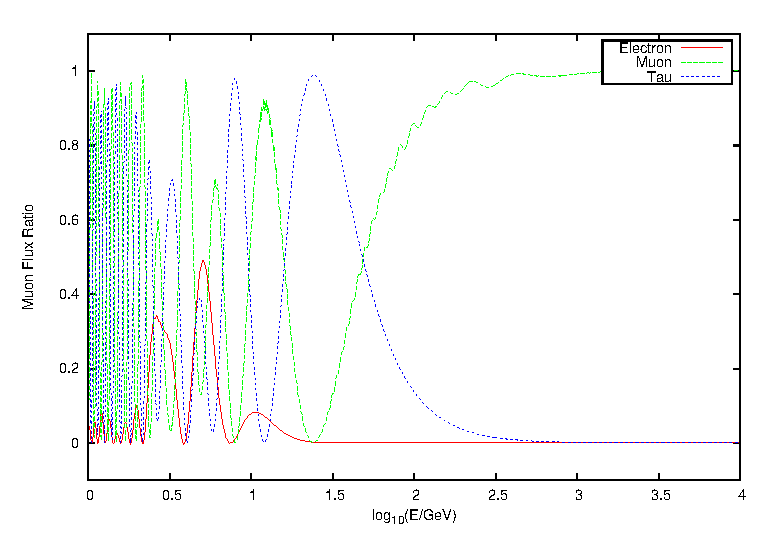
\includegraphics[width=0.7\textwidth]{fig/Multiplot.eps} 
  \caption{Output for the multiple energy mode with sterile neutrino (3+1)} 
\end{figure}
 
In fig.\ref{fig:multimode} we show the results of running this example
for the case with sterile neutrino.

\subsection{Read and Write \textnormal{({\ttf examples/HDF5\_Write\_Read})}}
\label{sec:readwrite}
In this example we illustrate the use of the functions to
read and write {\ttf HDF5} files. The file contains the full
information of the system: all settings, body, track (including
current position in the track), and the density matrix at each node.
This serialization allows to save the system
in the middle of a complex propagation and read it later to continue
the calculation. Saving the system using this and loading it from
the file restores the system to the saved state allowing the user to
compute any quantum mechanical observable.

This example is based upon the multiple energy example but
split in two parts. The first part computes the evolution and saves the
state of the system ({\ttf write.cpp}). The second reads the
state,  extract the flavor fluxes, and  prints them to a file ({\ttf
  read.cpp}).

In the following we describe lines that are relevant for reading and writing.

In the file {\ttf write.cpp} we save the system before and after the
evolution.
\begin{lstlisting}[frame=leftline, numbers =
  left,breaklines=true,label = ex:sin1]
  nus.WriteStateHDF5(``./initial_state.hdf5'');
  nus.EvolveState();
  nus.WriteStateHDF5(``./final_state.hdf5'');
\end{lstlisting}

And in order to recover that in the {\ttf read.cpp} file we use the
constructor that takes as an argument the name of the file.

\begin{lstlisting}[frame=leftline, numbers =
  left,breaklines=true,label = ex:sin1]
  nuSQUIDS inus(``./initial_state.hdf5'');
  nuSQUIDS fnus(``./final_state.hdf5''); 
\end{lstlisting}


\subsection{Construction and use of bodies \textnormal{({\ttf
      examples/Bodies})}}
\label{sec:body}
One of the main classes in the nuSQUIDS library are the body and the
track. These two do not have defaults in the code and always needs to
be specified.
In this example we show how to use the objects already implemented in
the library and also how to create some objects from the classes
already defined.

The folder {\ttf examples/Bodies/} contains a new body an track
definitions in the files {\ttf exBody.h} and {\ttf exBody.cpp}.
It also contains the file {\ttf main.cpp} whose main function 
uses all the already existing objects in nuSQUIDS and the new objects
of these examples.


\subsubsection{Construct a derived body}

Here is an example of how to define a derived object of the EarthAtm
body. In this simple case the object is just an earth model with some
parameters that weight the relative densities in the different layers
of the Earth's inner core, outer core, and mantel.

In order to implement it we suggest to do it inside the {\ttf nusquids}
namespace. We define a new class called {\ttf EarthMod}, which is a derived class of {\ttf
  EarthAtm}. Because of this the new class will have all the properties,
values, and functions of the parent class. 
\begin{lstlisting}[frame=leftline, numbers = left,breaklines=true,label = ex:sin1]
namespace nusquids{

class EarthMod: public EarthAtm{
public:
\end{lstlisting}

Our object constructors requires the following inputs:
based earth model file name ({\ttf earthmodel}), inner core weight
({\ttf frho1}), outer core weight ({\ttf frho2}), mantle weight ({\ttf
  frho3}).

\begin{lstlisting}[frame=leftline, numbers = left,breaklines=true,label = ex:sin1,firstnumber=last]
  EarthMod(std::string earthmodel, double frho1, double frho2, double
  frho3);
\end{lstlisting}
The function {\ttf Mod} allows to change the parameters ones the
object is already defined.
\begin{lstlisting}[frame=leftline, numbers =
  left,breaklines=true,label = ex:sin1,firstnumber=last]
  void  Mod(double frho1, double frho2, double frho3);
};

\end{lstlisting}

The implementation of the functions that set the density arrays with
the modified values are given in the files {\ttf exBody.cpp}.

\subsubsection{Use of the bodies}

In this part we will describe what is implemented in {\ttf
  main.cpp}.
This file defines a nuSQUIDS object and sets different bodies and
tracks. For each of these it evolves the system and shows the
probabilities in the screen.
For simplicity we use the single energy mode sec.~\ref{sec:single}, but the use of the body
and track would be the same for the multiple energy case.

First we construct the nuSQUIDS object for three neutrinos, then we set the
oscillation parameters and the neutrino energy.

\begin{lstlisting}[frame=leftline, numbers =
  left,breaklines=true,label = ex:sin1]
  nuSQUIDS nus(3,neutrino);
  nus.Set_MixingAngle(0,1,0.563942);
  nus.Set_MixingAngle(0,2,0.154085);
  nus.Set_MixingAngle(1,2,0.785398);
  nus.Set_SquareMassDifference(1,7.65e-05);
  nus.Set_SquareMassDifference(2,0.00247);
  nus.Set_CPPhase(0,2,0.0);
  squids::Const units;
  nus.Set_E(10.0*units.GeV);
\end{lstlisting}

\begin{enumerate}
\item {\ttf Earth}

The first example is the {\ttf Earth} body. In this case the track is
parametrized by the baseline of the experiment. Here we define the
body and track. For the track we need to specify the initial and final
position as well as the baseline. 
\begin{lstlisting}[frame=leftline, numbers =
  left,breaklines=true,label = ex:sin1,firstnumber=last]
  double baseline = 500.0*units.km;
  std::shared_ptr<Earth> earth = std::make_shared<Earth>();
  std::shared_ptr<Earth::Track> earth_track = std::make_shared<Earth::Track>(0.0,baseline,baseline);
\end{lstlisting}
And we set the Body and Track to the nuSQuIDS object.
\begin{lstlisting}[frame=leftline, numbers =
  left,breaklines=true,label = ex:sin1,firstnumber=last]
  nus.Set_Body(earth);
  nus.Set_Track(earth_track);
\end{lstlisting}

We first set the initial state of the system and print the state in
the screen.
\begin{lstlisting}[frame=leftline, numbers =
  left,breaklines=true,label = ex:sin1,firstnumber=last]
  marray<double,1> ini_state({3},{0,1,0});
  nus.Set_initial_state(ini_state,flavor);
  // Lets print out the initial state
  std::cout << "In state" << std::endl;
  for (double EE : nus.GetERange()){
    std::cout << EE/units.GeV << " ";
    for(int i = 0; i < 3; i++){
      std::cout << nus.EvalFlavor(i) << " ";
    }
    std::cout << std::endl;
  }
\end{lstlisting}
We set the numerical error and maximum step for the GSL integrator.
\begin{lstlisting}[frame=leftline, numbers =
  left,breaklines=true,label = ex:sin1,firstnumber=last]
  nus.Set_h_max( 200.0*units.km );
  nus.Set_rel_error(1.0e-12);
  nus.Set_abs_error(1.0e-12);
\end{lstlisting}

Finally we evolve the state and print in the screen the final state of
the system.
\begin{lstlisting}[frame=leftline, numbers =
  left,breaklines=true,label = ex:sin1,firstnumber=last]
  nus.EvolveState();
  std::cout << "Out state" << std::endl;
  for (double EE : nus.GetERange()){
    std::cout << EE/units.GeV << " ";
    for(int i = 0; i < 3; i++){
      std::cout << nus.EvalFlavor(i) << " ";
    }
    std::cout << std::endl;
  }
\end{lstlisting}
These last steps in the code are the same in all the bodies examples and we
are omitting this for the next cases.

\item {\ttf EarthAtm}

In this example we use the {\ttf EarthAtm} body. The
track is defined by the zenith angle of the trajectory.
\begin{lstlisting}[frame=leftline, numbers =
  left,breaklines=true,label = ex:sin1,firstnumber=last]
  double phi = acos(-1.0);
  std::shared_ptr<EarthAtm> earth_atm = std::make_shared<EarthAtm>();
  std::shared_ptr<EarthAtm::Track> earth_atm_track = std::make_shared<EarthAtm::Track>(phi);

  nus.Set_Body(earth_atm);
  nus.Set_Track(earth_atm_track);
\end{lstlisting}

\item {\ttf earth\_mod}

  In this case we use the modified earth object.
  As before the track is deffined by the zenith angle of
  the trajectory. In the constructor we set all the weight to $0.1$.
  Finally we set the body an track to nuSQUIDS.
  
\begin{lstlisting}[frame=leftline, numbers =
  left,breaklines=true,label = ex:sin1,firstnumber=last]
  double phi = acos(-1.0);
  std::shared_ptr<EarthMod> earth_mod = std::make_shared<EarthMod>(0.1,0.1,0.1);
  std::shared_ptr<EarthMod::Track> earth_mod_track = std::make_shared<EarthMod::Track>(phi);  

  nus.Set_Body(earth_mod);
  nus.Set_Track(earth_mod_track);
\end{lstlisting}


\item {\ttf VariableDensity}

In this case we use the variable density body and a track of $200{\rm km}$
First we define the density, position, and electron fraction arrays
with the corresponding values.
\begin{lstlisting}[frame=leftline, numbers =
  left,breaklines=true,label = ex:sin1,firstnumber=last]
  int N=40;

  std::vector<double> x_arr(N);
  std::vector<double> density_arr(N);
  std::vector<double> ye_arr(N);

  double size = 1000.0*units.km;
  for(int i = 0; i < N; i++){
    x_arr[i] = size*(i/(double)N);
    density_arr[i] = fabs(cos((double)i));
    ye_arr[i] = fabs(sin((double)i));
  }
\end{lstlisting}

Now we construct the body and the track. The constructor for the
variable density takes as an input the position, density, and electron
fraction vectors. Finally, like before, we set the body and the track in nuSQUIDS.
\begin{lstlisting}[frame=leftline, numbers =
  left,breaklines=true,label = ex:sin1,firstnumber=last]

  std::shared_ptr<VariableDensity> vardens = std::make_shared<VariableDensity>(x_arr,density_arr,ye_arr);
  std::shared_ptr<VariableDensity::Track> track_vardens = std::make_shared<VariableDensity::Track>(0.0,200.0*units.km);

  nus.Set_Body(vardens);
  nus.Set_Track(track_vardens);
\end{lstlisting}

\item {\ttf Vacuum}

This is a trivial case where the density and electron fraction are
zero. We only need to give the baseline as an argument to construct
the track. In this example we set the baseline to $500{\rm km}$.

\begin{lstlisting}[frame=leftline, numbers =
  left,breaklines=true,label = ex:sin1,firstnumber=last]
  double baseline_2 = 500.0*units.km;
  std::shared_ptr<Vacuum> vacuum = std::make_shared<Vacuum>();
  std::shared_ptr<Vacuum::Track> track_vac = std::make_shared<Vacuum::Track>(baseline_2);
  
  nus.Set_Body(vacuum);
  nus.Set_Track(track_vac);
\end{lstlisting}

\item {\ttf ConstantDensity}

In the case of constant density an analytic approximation can be
used to propagate the neutrinos if non-coherent interactions are
disabled in the construction of the nuSQuIDS object. The full
Hamiltonian of the system is diagonalized and exponentiated. 

We set the density to $100{\rm g/cm}^3$, the electron fraction to $0.3$, and the
baseline to $500{\rm km}$.
\begin{lstlisting}[frame=leftline, numbers =
  left,breaklines=true,label = ex:sin1,firstnumber=last]

  double density = 100.0;
  double ye = 0.3;
  std::shared_ptr<ConstantDensity> constdens = std::make_shared<ConstantDensity>(density,ye);
  double baseline_3 = 500.0*units.km;
  std::shared_ptr<ConstantDensity::Track> track_constdens =   std::make_shared<ConstantDensity::Track>(0.0,baseline_3);

  nus.Set_Body(constdens);
  nus.Set_Track(track_constdens);
\end{lstlisting}
\end{enumerate}

\subsection{Cross Sections \textnormal{({\ttf
      examples/Xsections})}}

One of the important features of nuSQuIDS is the possibility of handling in a
consistent way the non-coherent interactions with the oscillation
behavior. The physical quantity that encodes how often this scattering
interaction happen between the neutrinos and the media is the cross
section.
nuSQuIDS it has implemented two kind of interactions: charge and
neutral current. In the case of charge current we have in to account
the neutrinos produced by the decay of short lived charged particles
such as $\tau$ and $W^\pm$. For the neutral current we always include
the outgoing neutrino.
Other particles produced in the interactions such as hadrons or long
lived charged leptons are ignored along the evolution.
This information is organized and stored in the cross-section class.
This class requires the user to provide the total cross-section for
each flavor and current in units of cm$^2$. It also requires to
specify the single differential neutrinos cross sections with respect to
the outgoing neutrino energy in units of cm$^2$/GeV. 

nuSQuIDS includes by default deep inelastic neutrino nucleon
cross-sections as well as neutrino electron
cross-sections~\citep{Gandhi:1998ri, CooperSarkar:2011pa}.

In this example construct a new cross section object to be used by
nuSQuIDS instead of the default one.
Every cross section must be a class of {\ttf NeutrinoCrossSections}
and implement at least two member functions:
{\ttf SingleDifferentialCrossSection} and {\ttf TotalCrossSection}.


\begin{lstlisting}[frame=leftline, numbers =
  left,breaklines=true,label = ex:sin1]
  class LinearCrossSections : public NeutrinoCrossSections {
    private:
    const squids::Const units;
    const double GF = 1.16639e-23; // eV^-2
    const double mp = 938.272e6; // proton mass eV
    const double CC_to_NC; // proportion of CC to NC which goes from 0 to 1.
    public :
    LinearCrossSections(double CC_to_NC):CC_to_NC(CC_to_NC){assert( CC_to_NC <= 1.0  && CC_to_NC >= 0.0 );}
    LinearCrossSections():LinearCrossSections(0.5){}
    double TotalCrossSection(double Enu, NeutrinoFlavor flavor, NeutrinoType neutype, Current current) const override;
    double SingleDifferentialCrossSection(double E1, double E2, NeutrinoFlavor flavor, NeutrinoType neutype, Current current) const override;
  };  
 
\end{lstlisting}

In this example we use a toy total cross section that scales linearly with
the neutrino energy and the corresponding differential cross sections
linear in the outgoing neutrino energy; see implementation in {\ttf
  exCross.cpp}. We also allow to change the proportion charge to
neutral current at the construction of the object.


We construct two cross section objects: one with only charge current  interactions
{\ttf ncs\_cc} and another with only neutral current {\ttf
  ncs\_nc}. Then we construct the corresponding nuSQuIDS objects {\ttf nus\_cc} and {\ttf nus\_nc}.
We also disable neutrino oscillations in this example by means of the
option {\ttf Set\_IncludeOscillations(false)}.

\begin{lstlisting}[frame=leftline, numbers =  
  left,breaklines=true,label = ex:sin1]
  std::shared_ptr<NeutrinoCrossSections> ncs_cc=std::make_shared<LinearCrossSections>(0.0);
  std::shared_ptr<NeutrinoCrossSections> ncs_nc=std::make_shared<LinearCrossSections>(1.0);

  nuSQUIDS nus_cc(logspace(Emin,Emax,200),numneu,neutrino,true,ncs_cc);
  nus_cc.Set_IncludeOscillations(false);
  nuSQUIDS nus_nc(logspace(Emin,Emax,200),numneu,neutrino,true,ncs_nc);
  nus_nc.Set_IncludeOscillations(false);
\end{lstlisting}


We can see the final to initial flux ratios for both cases in fig~\ref{fig:crossext}.

\begin{figure}[h!]
  \label{fig:crossext}
  \centering
  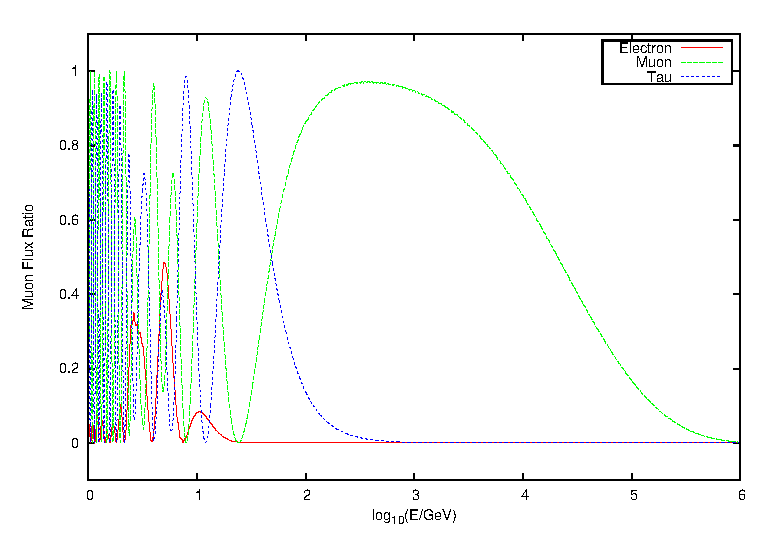
\includegraphics[width=0.7\textwidth]{fig/crossext.eps} 
  \caption{Final to initial flux ratio as a function of the logarithm
    of the neutrino energy for the example toy cross sections with
    only charged current and only neutral current.} 
\end{figure}


\subsection{Constant density multiple layers \textnormal{({\ttf
      examples/Constant\_density\_layers})}}
Since the constant density allows us to do very fast computation using
the diagonalization of the full Hamiltonian here we show an example
where we concatenate the evolution of the neutrinos through different
layers of constant density.

We construct three different layers: first $100{\rm km}$ in
vacuum, second $50{\rm km}$ in matter with density $3.5{\rm g/cm}^3$ and
 electron fraction $0.5$, and finally $200{\rm km}$ in matter with
 density $10{\rm g/cm}^3$ and electron fraction $0.1$.
 
\begin{lstlisting}[frame=leftline, numbers =
  left,breaklines=true,label = ex:sin1]
  const double layer_1 = 100.*units.km;
  std::shared_ptr<Vacuum> vacuum = std::make_shared<Vacuum>();
  std::shared_ptr<Vacuum::Track> track_env0 = std::make_shared<Vacuum::Track>(layer_1);

  const double layer_2 = 50.*units.km;
  std::shared_ptr<ConstantDensity> constdens_env1 = std::make_shared<ConstantDensity>(3.5,0.5); 
  std::shared_ptr<ConstantDensity::Track> track_env1 = std::make_shared<ConstantDensity::Track>(layer_2);

  const double layer_3 = 200.*units.km;
  std::shared_ptr<ConstantDensity> constdens_env2 = std::make_shared<ConstantDensity>(10.,0.1);
  std::shared_ptr<ConstantDensity::Track> track_env2 = std::make_shared<ConstantDensity::Track>(layer_3);
\end{lstlisting}

Now in order to evolve the system we set the corresponding body
and track and evolve every layer.

\begin{lstlisting}[frame=leftline, numbers =
  left,breaklines=true,label = ex:sin1]
  nus.Set_Body(vacuum);
  nus.Set_Track(track_env0);
  nus.EvolveState();

  nus.Set_Body(constdens_env1);
  nus.Set_Track(track_env1);
  nus.EvolveState();

  nus.Set_Body(constdens_env2);
  nus.Set_Track(track_env2);
  nus.EvolveState();
\end{lstlisting}

Finally, we write the output for the different flavor fluxes in a text file.


\subsection{BSM extension: Non-Standard  Interaction (NSI) \textnormal{({\ttf
      examples/NSI})}}
\label{sec:NSI}
In this example we illustrate how to construct a derived class of
nuSQuIDS including a new physics term. This procedure is similar to
other new physics setups~\ref{sec:LV}.

The implementation of {\ttf nuSQUIDSNSI} class is in {\ttf NSI.h}.
We will go trough the implementation to see what needs to be
added to be base class.

First, we declare the NSI matter potential as a {\ttf SU\_vector}
called {\ttf NSI}. By default nuSQuIDS  works in the interaction
picture, thus every term we add to the hamiltonian has to be properly
evolved with $H_0$. Since $H_0$ depends on the energy to do this in
every node. For optimization we will compute and store the evolved NSI
term in a vector of {\ttf SU\_vector} objects called {\ttf NSI\_evol}.

The {\ttf HI\_prefactor} contains all the numerical factors multiplying the
operator and {\ttf epsilon\_mutau} is the strength of the NSI $\mu$-$\tau$ 
non-diagonal component. Notice that we set all other NSI
contributions to zero.

\begin{lstlisting}[frame=leftline, numbers =
  left,breaklines=true,label = ex:sin1]
class nuSQUIDSNSI: public nuSQUIDS {
  private:
    squids::SU_vector NSI;
    std::vector<squids::SU_vector> NSI_evol;
    std::unique_ptr<double[]> hiBuffer;
    double HI_prefactor;
    // nsi parameters
    double epsilon_mutau;

\end{lstlisting}

As we said before we need to compute the NSI operator in the
interaction picture prior to adding it to the r.h.s. of the
differential equation. We compute this for every energy node in the
{\ttf AddToPreDerive} function. This function is called inside the
{\ttf PreDerive} function before evaluating the derivatives to allow
the user to pre-compute terms used in the derivative.
The evolution of the NSI term by $H_0$ is done by the {\ttf
  SU\_vector::Evolve} member. This function is optimized and performs
the evolution of the operator analytically.

\begin{lstlisting}[frame=leftline, numbers =
  left,breaklines=true,label = ex:sin1,firstnumber=last]
    void AddToPreDerive(double x){
      for(int ei = 0; ei < ne; ei++){
        NSI_evol[ei] = NSI.Evolve(H0_array[ei],(x-Get_t_initial()));
      }
    }
\end{lstlisting}

The following auxiliary member functions allow {\ttf nuSQUIDSNSI} to
save the new physics parameters into the hdf5 files when the
{\ttf WriteStateHDF5} is called~\ref{sec:readwrite}.

\begin{lstlisting}[frame=leftline, numbers =
  left,breaklines=true,label = ex:sin1,firstnumber=last]
    void AddToReadHDF5(hid_t hdf5_loc_id){
      // here we read the new parameters now saved in the HDF5 file
      hid_t nsi = H5Gopen(hdf5_loc_id, "nsi", H5P_DEFAULT);
      H5LTget_attribute_double(hdf5_loc_id,"nsi","mu_tau" ,&epsilon_mutau);
      H5Gclose(nsi);
    }

    void AddToWriteHDF5(hid_t hdf5_loc_id) const {
      // here we write the new parameters to be saved in the HDF5 file
      H5Gcreate(hdf5_loc_id, "nsi", H5P_DEFAULT, H5P_DEFAULT, H5P_DEFAULT);
      H5LTset_attribute_double(hdf5_loc_id, "nsi","mu_tau",&epsilon_mutau, 1);
    }
\end{lstlisting}

Here we overload the {\ttf HI} function where we return the nuSQuIDS
matter potential plus the new NSI contribution.

\begin{lstlisting}[frame=leftline, numbers =
  left,breaklines=true,label = ex:sin1,firstnumber=last]
    squids::SU_vector HI(unsigned int ei,unsigned int index_rho) const{
      double CC = HI_prefactor*body->density(*track)*body->ye(*track);

      squids::SU_vector potential(nsun,hiBuffer.get());

      potential = (3.0*CC)*NSI_evol[ei];

      if ((index_rho == 0 and NT==both) or NT==neutrino){
          return nuSQUIDS::HI(ei,index_rho) + potential;
      } else if ((index_rho == 1 and NT==both) or NT==antineutrino){
          return nuSQUIDS::HI(ei,index_rho) + (-1.0)*std::move(potential);
      } else{
          throw std::runtime_error("nuSQUIDS::HI : unknown particle or antiparticle");
      }
    }
\end{lstlisting}

The constructor first calls the
nuSQUIDS constructor and then sets the oscillation
paramters and the NSI operator.

\begin{lstlisting}[frame=leftline, numbers =
  left,breaklines=true,label = ex:sin1,firstnumber=last]
  public:
  nuSQUIDSNSI(double epsilon_mutau, marray<double,1> Erange,
              int numneu, NeutrinoType NT, bool iinteraction,
              double th01=0.563, double th02=0.154, double th12=0.785):
              nuSQUIDS(Erange,numneu,NT,iinteraction),
	      hiBuffer(new double[nsun*nsun]),
              epsilon_mutau(epsilon_mutau)
  {
    assert(numneu == 3);
    // defining a complex matrix M which will contain our flavor
    // violating flavor structure.
    gsl_matrix_complex * M = gsl_matrix_complex_calloc(3,3);
    gsl_complex c {{ epsilon_mutau , 0.0 }};
    gsl_matrix_complex_set(M,2,1,c);
    gsl_matrix_complex_set(M,1,2,gsl_complex_conjugate(c));
    
    NSI = squids::SU_vector(M);
    
    Set_MixingAngle(0,1,th01);
    Set_MixingAngle(0,2,th02);
    Set_MixingAngle(1,2,th12);
    
    // rotate to mass reprentation
    NSI.RotateToB1(params);
    NSI_evol.resize(ne);
    for(int ei = 0; ei < ne; ei++){
      NSI_evol[ei] = squids::SU_vector(nsun);
    }
    gsl_matrix_complex_free(M);
    
    HI_prefactor = params.sqrt2*params.GF*params.Na*pow(params.cm,-3);
  }
\end{lstlisting}

The next function sets the value of {\ttf epsilon\_mutau} changing the
 {\ttf SU\_vector NSI} object accordingly. We construct the {\ttf
   SU\_vector} operator as a complex GSL matrix that represents the
 operator in the flavor basis. Since nuSQuIDS solves the propagation
 in the basis where $H_0$ is diagonal, i.e. the mass basis, we rotate
 the NSI operator to the mass basis by calling {\ttf RotateToB1}.

\begin{lstlisting}[frame=leftline, numbers =
  left,breaklines=true,label = ex:sin1,firstnumber=last]
  void Set_mutau(double eps){
    gsl_matrix_complex * M = gsl_matrix_complex_calloc(3,3);
    gsl_complex c {{ epsilon_mutau , 0.0 }};
    gsl_matrix_complex_set(M,2,1,c);
    gsl_matrix_complex_set(M,1,2,gsl_complex_conjugate(c));
    NSI = squids::SU_vector(M);    
    NSI.RotateToB1(params);
    gsl_matrix_complex_free(M);
  }
\end{lstlisting}

In {\ttf main.cpp} we use the new NSI in a
multiple energy mode. In order to compare the oscillation
probabilities with and without NSI we construct two instances {\ttf
  nuSQUIDSNSI} with {\ttf  epsilon\_mutau=0} and {\ttf
  epsilon\_mutau=1e-2}. 

\begin{lstlisting}[frame=leftline, numbers =
  left,breaklines=true,label = ex:sin1,firstnumber=last]
  double eps_mutau=1.0e-2;
  nuSQUIDSNSI nus(eps_mutau,logspace(Emin,Emax,200),numneu,antineutrino,false);
  nuSQUIDSNSI nus_zero(0.0,logspace(Emin,Emax,200),numneu,antineutrino,false);
\end{lstlisting}

In the next lines we propagate both objects and print both
fluxes in a file.

\begin{lstlisting}[frame=leftline, numbers =
  left,breaklines=true,label = ex:sin1,firstnumber=last]
  nus.EvolveState();
  nus_zero.EvolveState();

  int Nen =1000;
  double lEmin=log10(Emin);
  double lEmax=log10(Emax);
  
  std::ofstream file("fluxes_flavor.txt");

  file << "# log10(E) E flux_NSI_i flux_noNSI_i . . . ." << std::endl;
  for(double lE=lEmin; lE<lEmax; lE+=(lEmax-lEmin)/(double)Nen){
    double E=pow(10.0,lE);
    file << lE << " " << E << " ";
    for(int fl=0; fl<numneu; fl++){
      file << " " <<  nus.EvalFlavor(fl, E) << " " <<  nus_zero.EvalFlavor(fl, E);
    }
    file << std::endl;
  }
\end{lstlisting}

In the folder there is a script that allows to plot the output text
file.


\subsection{BSM extension: Lorentz Violation \textnormal{({\ttf
      examples/LV})}}
The Lorentz symmetry is a well established property of space-time.
As a fundamental symmetry it should be tested and neutrino
oscillations prove part of the parameter space.

The example is technically the same as the non-standard interactions,
but we add a couple of features illustrate good practices.

As before the new term is added in to {\ttf HI}. For this particular
physics case the effect is positive for neutrinos and negative for
antineutrinos. This can be implemented using the integer {\ttf irho}
which labels neutrinos with $0$ and antineutrinos with $1$.

\begin{lstlisting}[frame=leftline, numbers =
  left,breaklines=true,label = ex:sin1,firstnumber=last]
  squids:: SU_vector HI(unsigned int ie,unsigned int irho) const {
    squids::SU_vector potential = nuSQUIDS::HI(ie, irho);
    double sign = 1;
    if ((irho == 1 and NT==both) or NT==antineutrino){
      // antineutrino matter potential flips sign
      sign*=(-1);
    }
    // ===== HERE WE ADD THE NEW PHYSICS =====
    potential += sign*pow(E_range[ie],n_)*LVP_evol[ie]; 
    // ===== HERE WE ADD THE NEW PHYSICS =====
    return potential;
  }
\end{lstlisting}

The parameters of the Lorentz violating term is set by the function
{\ttf Set\_LV\_OpMatrix}. In doing that the oscillation parameters are
used to rotate to the mass basis. Therefore any change done in the
oscillation parameters after setting the LV term will be inconsistent.
In order to prevent inconsistencies we overload the function that sets
the mixing parameters {\ttf Set\_MixingAngle} and the phases {\ttf
  Set\_CPPhase} turning the label {\ttf lv\_parameters\_set} to {\ttf
  false} and forcing the need to call {\ttf Set\_LV\_OpMatrix} again.
This enforces the order of the set functions calls.

\begin{lstlisting}[frame=leftline, numbers =
  left,breaklines=true,label = ex:sin1,firstnumber=last]
    void Set_MixingAngle(unsigned int i, unsigned int j,double angle){
      nuSQUIDS::Set_MixingAngle(i,j,angle);
      lv_parameters_set = false;
    }

    void Set_CPPhase(unsigned int i, unsigned int j,double angle){
      nuSQUIDS::Set_CPPhase(i,j,angle);
      lv_parameters_set = false;
    }
\end{lstlisting}

\subsection{Decoherence or averaged oscillations\\ \textnormal{({\ttf
      examples/Astrophysical\_neutrino\_flavor\_ratio})}}

This file demonstrates how to the astrophysical flavo ratio by means
of using the averaged out approximation. We do this in two ways in this
example: first explicitly using the PMNS matrix and the formula given
in the literature and second by means of nuSQuIDS fast averaging functionality.
For simplicity we will do this example in the single energy mode, but it
can be performed in the multiple energy mode too.


In this example we set {\ttf N\_neutrino = 3} and {\ttf Type = "neutrino"}.

\begin{lstlisting}[frame=leftline, numbers =
  left,breaklines=true,label = ex:sin1]
  nuSQUIDS nus(3,neutrino);
\end{lstlisting}

We use the standard parametrization.

\begin{lstlisting}[frame=leftline, numbers =
  left,breaklines=true,label = ex:sin1]
  nus.Set_MixingAngle(0,1,0.563942);
  nus.Set_MixingAngle(0,2,0.154085);
  nus.Set_MixingAngle(1,2,0.785398);

  nus.Set_SquareMassDifference(1,7.65e-05);
  nus.Set_SquareMassDifference(2,0.00247);
  
  nus.Set_CPPhase(0,2,0.0);
\end{lstlisting}

We construct and set the body and the track, in this case we use vacuum
oscillations.

\begin{lstlisting}[frame=leftline, numbers =
  left,breaklines=true,label = ex:sin1]
  std::shared_ptr<Vacuum> vacuum = std::make_shared<Vacuum>();
  std::shared_ptr<Vacuum::Track> vacuum_track = std::make_shared<Vacuum::Track>(1.e3*units.kparsec);
  nus.Set_Body(vacuum);
  nus.Set_Track(vacuum_track);
\end{lstlisting}

Here we set the initial state for the flavor, a pion produced flavor composition

\begin{lstlisting}[frame=leftline, numbers =
  left,breaklines=true,label = ex:sin1]
  marray<double,1> ini_state({3},{1,2,0});
  nus.Set_initial_state(ini_state,flavor);
\end{lstlisting}

We evolve the neutrinos.

\begin{lstlisting}[frame=leftline, numbers =
  left,breaklines=true,label = ex:sin1]
  nus.EvolveState();
\end{lstlisting}

nuSQuIDS can calculate the average oscillation probability
where the oscillation frequencies are larger than some value
we call this value {\ttf scale}. When this mode is used its often
valuable to know which frequencies have been averaged out.
NuSQuIDS this by sting true a boolean vector {\ttf is\_avg} provided to the
evaluation function.

\begin{lstlisting}[frame=leftline, numbers =
  left,breaklines=true,label = ex:sin1]
  nus.EvolveState();
  double scale = 0.;
  std::vector<bool> is_avg(3);
\end{lstlisting}

The get the result always averaged we can set the scale to the maximum
double numerical limit.

\begin{lstlisting}[frame=leftline, numbers =
  left,breaklines=true,label = ex:sin1]
  scale = std::numeric_limits<double>::max();
\end{lstlisting}

We output the result for the averaged and non averaged computations.

\begin{lstlisting}[frame=leftline, numbers =
  left,breaklines=true,label = ex:sin1]
    std::cout << "Out state" << std::endl;
  for (double EE : nus.GetERange()){
    std::cout << EE/units.GeV << " ";
    for(int i = 0; i < 3; i++){
      std::cout << nus.EvalFlavor(i, scale, is_avg);
      std::cout << " (" << (is_avg[i] ? "avg." : "no avg.")  << ") ";
    }
    std::cout << std::endl;
  }

  scale = 0.0;

  std::cout << "Out state" << std::endl;
  for (double EE : nus.GetERange()){
    std::cout << EE/units.GeV << " ";
    for(int i = 0; i < 3; i++){
      std::cout << nus.EvalFlavor(i, scale, is_avg);
      std::cout << " (" << (is_avg[i] ? "avg." : "no avg.")  << ") ";
    }
    std::cout << std::endl;
  }
\end{lstlisting}

Notice that the average calculation is done only on the
oscillations given by $H_0$ when any oscillation is evaluated. Fast
oscillations from other terms, such $H_I$  wont be
averaged out.


\subsection{Atmospheric Mode: Standard \textnormal{({\ttf
      examples/Atm\_default})}}
\label{sec:atmexample}
In this example we show how to use the atmospheric mode. This mode is
a compact way to treat a set of nuSQUIDS objects distributed in
zenith.
This allows us to propagate the energy-zenith dependent atmospheric
neutrino flux thought the Earth.

First, we construct the nuSQUIDSAtm object. The parameters of the
constructors are the list of cosine of the zenith angle values ({\ttf
  linspace(czmin,czmax,40)}) and the following arguments as the
multiple energy constructor.

\begin{lstlisting}[frame=leftline, numbers =
  left,breaklines=true,label = ex:sin1]
  double Emin=1.e1*units.GeV;
  double Emax=1.e6*units.GeV;
  double czmin=-1;
  double czmax=0;

  nuSQUIDSAtm<> nus_atm(linspace(czmin,czmax,40),logspace(Emin,Emax,100),numneu,both,interactions);
\end{lstlisting}

In this case the initial state is marray of rank four with double values.  
The first index is for the zenith, the second for the energy, the
third for particle type (neutrino or antineutrino), and the last one
for the neutrino flavor.

In this example we fill the multi-dimensional array with the initial state of the
system where the function {\ttf flux\_function} would be the corresponding
atmospheric flux.

\begin{lstlisting}[frame=leftline, numbers =
  left,breaklines=true,label = ex:sin1,firstnumber=last]
  marray<double,4> inistate{nus_atm.GetNumCos(),nus_atm.GetNumE(),2,numneu};
  std::fill(inistate.begin(),inistate.end(),0);
  for ( int ci = 0 ; ci < nus_atm.GetNumCos(); ci++){
    for ( int ei = 0 ; ei < nus_atm.GetNumE(); ei++){
      for ( int rho = 0; rho < 2; rho ++ ){
        for (int flv = 0; flv < numneu; flv++){
          inistate[ci][ei][rho][flv] = (flv == 1) ? flux_function(e_range[ei], cz_range[ci]) : 0.0;//set 1 only to the muon flavor
        }
      }
    }
  }
  nus_atm.Set_initial_state(inistate,flavor);
\end{lstlisting}

To evolve the full state we call as always {\ttf EvolveState}. 

\begin{lstlisting}[frame=leftline, numbers =
  left,breaklines=true,label = ex:sin1,firstnumber=last]
nus_atm.EvolveState();
\end{lstlisting}

Finally, we evaluate as print the flux in a file. The
atmospheric mode has an interpolation implemented that allows to
evaluate the flux at any flavor, energy, and cosine-zenith. See \ref{sec:atm}
for more details.


\begin{lstlisting}[frame=leftline, numbers =
  left,breaklines=true,label = ex:sin1,firstnumber=last]
  int Nen=700;
  int Ncz=100;
  double lEmin=log10(Emin);
  double lEmax=log10(Emax);;

  file << "# log10(E) cos(zenith) E flux_i . . . ." << std::endl;
  for(double cz=czmin;cz<czmax;cz+=(czmax-czmin)/(double)Ncz){
    for(double lE=lEmin; lE<lEmax; lE+=(lEmax-lEmin)/(double)Nen){
      double E=pow(10.0,lE);
      file << lE << " " << cz << " " << E;
      for(int fl=0; fl<numneu; fl++){
	file << " " <<  nus_atm.EvalFlavor(fl,cz, E);
      }
      file << std::endl;
    }
    file << std::endl;
  }
\end{lstlisting}


\subsection{Atmospheric mode: BSM \textnormal{({\ttf examples/Atm\_BSM})}}
\label{sec:atmBSM}
The atmospheric mode is implemented such  that it can be used with any
nuSQUIDS derived class. In this example we use the atmospheric mode
with the NSI nuSQUIDS extension shown in the NSI example~\ref{sec:NSI}.

In the folder we include a copy of the NSI header file {\ttf NSI.h}.
The main file is essentially the same as the atmospheric default mode
example with the following changes.
The class type template argument is the nuSQuIDS derived class. The
constructor takes list of cosine zenith angle values and then the
derived class constructor arguments. 

\begin{lstlisting}[frame=leftline, numbers =
  left,breaklines=true,label = ex:sin1,firstnumber=last]
  double epsilon_mutau=1e-2;
  nuSQUIDSAtm<nuSQUIDSNSI> nus_atm(linspace(czmin,czmax,40),epsilon_mutau,logspace(Emin,Emax,100),numneu,both,true);
\end{lstlisting}

\section{Performance and precision}
\label{sec:performance} 

Machine 1 is configured with an Intel 6700K CPU, with a `base' frequency of 4.0 GHz. All tests were performed with the `Turbo Boost' feature disabled. 

The time evolution and basis transformations performed by SQuIDS on SU\_vector objects rely heavily on trigonometric functions, specifically sines and cosines, mostly in matched pairs. These operations are in turn used by several of the key portions of nuSQuIDS, and for oscillation-only calculations evaluation of trigonometric functions can be the single largest part of time consumed by the library. As a result, run time is strongly dependent on the performance of the underlying math library, which is usually supplied by the operating system, and sometimes the compiler. The considerable differences which can result are illustrated in Table $\ref{tab:trig_perf}$, which shows measurements performed on Machine 1 with several combinations of operating system and compiler of the cost of computing a single sine function or the combination of sine and cosine for the same argument (which should ideally be performed by an efficient, fused calculation). A measurement was also made of the time to run the pseudo-random number generator (PRNG) by itself. The time spent for the PRNG varies somewhat, assumedly due to different optimization choices by the various compilers, but amounts to a small fraction of the time for the trigonometric calculation is included. Broadly, it is apparent that the calculations using the math implementations from the GNU C Library (glibc) library are significantly slower than the versions using other math libraries. Furthermore, the glibc calculations appear to benefit only slightly from the opportunity to fuse sine and cosine calculations; while they are not as slow as might be expected from a simple doubling of the time to compute a single sine they are also not much better. This is contrast to the other implementations which are able to compute both functions in essentially the same time as a single function (or with relatively low overhead, in the case of BSD libc). In addition to this overhead, the glibc time to compute a single trigonometric function is approximately twice that of the other libraries (it is unclear why the result is far worse for clang 5.0.1 on CentOS 7, but this was deemed to have little practical relevance to this work and was not further investigated). Unfortunately, the conclusion is that the choice of compiler can be extremely important to maximizing the performance of nuSQuIDs. The benchmarks shown in this section will use the Intel compiler, version 18.0.3 on Cent OS 7, unless otherwise noted. 

\begin{table*}
	\begin{tabular}{ llcccl }
		OS & Compiler & PRNG & Sine & Sine \& Cosine & Math Library \\
		CentOS 7 & gcc 4.8.5 & 6.0 ns & 40.5 ns & 63.5 ns & GNU C Library  2.17 \\
		CentOS 7 & gcc 7.3.1 & 2.7 ns & 37.1 ns & 63.3 ns & GNU C Library  2.17 \\
		CentOS 7 & clang 5.0.1 & 4.8 ns & 96.4 ns & 69.0 ns & GNU C Library  2.17 \\
		CentOS 7 & icc 18.0.3 & 4.0 ns & 20.9 ns & 22.2 ns & libimf 2018.3.222\\
		Darwin 16.7.0 & clang 5.0.0 & 2.9 ns & 19.1 ns & 20.1 ns & libsystem\_m  3121.6.0 \\
		FreeBSD 11.2 & clang 6.0.1 & 2.9 ns & 22.3 ns & 30.8 ns & BSD libc
	\end{tabular}
	\caption{
		Measured time to compute trigonometric functions using different compilers and operating systems. In each case the same stream of $10^8$ pseudo-random arguments in the domain [-100,100] was used, and the average time per call was computed, including the time necessary for the PRNG to compute the next argument value. 
	}
	\label{tab:trig_perf}
\end{table*}

\section{Test suite}
\label{sec:tests}
A test suit is provided with the library to warranty the right
performance in different systems or after any modification of the
code. All the test are located in the folder {\ttf nuSQuIDS/test}
And they can be run using the provided script {\ttf test/run\_tests}.
A single test can be run adding the name as and argument to the script
command.
In the following we list the tests that are provided with a brief
description of what they test.

\begin{itemize}
  
\item {\ttf test/vacuum\_osc\_prob.test}
  
  Tests that propagation with only oscillation of
  neutrinos in vacuum is equal to the analytic solution.

\item {\ttf test/constant\_density\_osc\_prob.test}
  
  Tests that propagation with only oscillation of
  neutrinos in constant density is equal to the analytic solution.

\item {\ttf test/constant\_opacity.test}
  
  Tests that propagation on a constant density with no oscillation and
  neglecting regeneration from neutral current or tau decay matches
  the expected expnential behavior.
  
\item {\ttf test/constant\_opacity\_with\_nc.test}
  
  Tests that propagation on a constant density with no oscillation 
  matches an independent numerical solution.  
  
\item {\ttf test/atmospheric\_he.test}

  Tests that the high-energy propagation without oscillation of
  neutrinos from the atmosphere does not give negative or {\ttf nan} values.

\item {\ttf test/atmospheric\_osc.test}
  
  Tests that propagation with only oscillation of
  neutrinos from the atmosphere does not give negative or {\ttf nan}
  values.
  
\item {\ttf test/body\_serialization.test}
  
  It checks that writing a body in to the hdf5 file and reading it
  back does not alter the body.  

\item {\ttf test/cross\_section\_consistency.test}
  
  Check that the differential cross section add with numerical error
  the total cross section.
  
\item {\ttf test/earth\_osc\_prob.test}
  
  Test that three and four neutrinos oscillation probability over a
  1000km baseline in multiple and single energy modes matches with the
  numerical error to reference independent calculation.
  
\item {\ttf test/glashow\_resonance.test}
  
  Checks that Glashow resonance integrated differential cross-section
  matches with the total cross-section and that is used while propagating. 
  
\item {\ttf test/hdf5\_atm\_in\_out.test}
  
  It checks that writing a nuSQuIDs atmospheric object into a hdf5 file and reading it
  back does not alter the object and recovers all the properties.

  
\item {\ttf test/hdf5\_in\_out.test}
  
  It checks that writing a nuSQuIDs object into a hdf5 file and reading it
  back does not alter the object and recovers all the properties.

\item {\ttf test/move\_assig.test}
  
  Checks that constructor of a nuSQuIDS object from an rvalue nuSQuIDS object works.
  
\item {\ttf test/mul\_energy\_constructor.test}
  
  Checks that the multiple energy constructor works.
  
\item {\ttf test/time\_reversal.test}
  
  Checks that propagating a neutrino and propagating again backwards
  in time returns to the original state.
  
\item {\ttf test/tools\_integrator.test}
  
  Checks that the provided one dimensional integrate function works
  with in the numerical error.
  
\item {\ttf test/track\_concatenate\_hdf5.test}
  
  Checks that propagating by concatenating a series of tracks in
  vacuum and writing and reading that state a every step is the same
  as propagating with a single track with the total length. 
  
  
\item {\ttf test/track\_concatenate.test}
  
  Checks that propagating by concatenating a series of tracks in
  vacuum is the same as propagating with a single track with the total length. 
  

\end{itemize}


\section{Description of the code} 
\label{sec:code} 

$\nu$-SQuIDS is a {\ttf C++} code built using the SQuIDS
framework \citep{SQUIDS}. It is designed to propagate neutrinos
through media while taking into account flavor oscillations and
non-coherent interactions. 

In order to allow the user to compute simple oscillation probabilities
for a single neutrino energy the code has a simplified mode.
In this mode the neutrino energy is fixed and only coherent interactions
are treated.
In this case, only Eq. \eqref{eq:schrodinger} is relevant for the
neutrino propagation, and the {\ttf nuSQuIDS} class implements {\ttf
  SQuIDS::H0} as in Eq. \eqref{eq:h0} and {\ttf SQuIDS::HI} as given
in Eq. \eqref{eq:hi}. 

In the default mode a statistical ensemble of neutrinos is
considered. The ensemble is described by means of a set of {\ttf
  SU\_vector} objects located at fixed  energy nodes spaced over the
energy region under consideration. Besides defining {\ttf SQuIDS::H0}
and {\ttf SQuIDS::HI}, as in the simplified single energy mode, the
following functions are also defined: {\ttf SQuIDS::GammaRho} by
equations \eqref{eq:gammarhoa} and \eqref{eq:gammarhob}, and {\ttf
  SQuIDS::InteractionsRho} in equations \eqref{eq:Fterm} and
\eqref{eq:antiFterm}. Furthermore, in the latter equation
\eqref{eq:antiFterm} $\tau$-regeneration is implemented assuming
instantaneous $\tau$ decay.

While the {\ttf nuSQuIDS} class implements all the necessary
differential equations, one must also specify the neutrino propagation
environment, propagation trajectory, and the relevant cross-sections.  
When interactions are considered the {\ttf nuSQuIDS} instance
will automatically construct appropriate {\ttf NeutrinoCrossSections}
and {\ttf TauDecaySpectra} objects to evaluate cross sections and
$\tau$ physics respectively. However, the user can also replace these
default versions if desired. The user must
explicitly specify the neutrino propagation medium and trajectory
through relevant specialization of {\ttf Body} and {\ttf Body::Track}.
Several implementations of {\ttf Body} and {\ttf Track} covering
common physics cases are supplied with the library. 

Finally, {\ttf nuSQuIDS} provides a set functions to evaluate the
neutrino ensemble flavor and mass composition. The code also have the
capability to store the system state in an HDF5~\citep{folk1999hdf5}
file for later use.

% TODO: mention setting mixing parameters used for propagation
\subsection{Body \& Track}

{\ttf Body} and {\ttf Body::Track} are abstract {\ttf C++} classes
which are used to represent the environment in which neutrinos
are propagated ({\ttf Body}) and the propagation path inside it ({\ttf
  Body::Track}). We will frequently use the shorthand {\ttf Track} for {\ttf Body::Track},
 when it should be clear from context that this is the type of {\ttf Track} 
 corresponding to a particular implementation of {\ttf Body}.

The evolution of the system depends on a single parameter which is
{\ttf double} member of {\ttf Track}. The
interplay between the evolution of this parameter and the trajectory
inside a given body is what is encoded in the {\ttf Body} and 
{\ttf Body::Track} classes. 
Namely, a {\ttf Body} is defined as a matter density and electron
fraction depending on the position in a 3 dimensional space, $\rho_m(\vec{r})$ and
$Y_e(\vec{r})$, the role of the {\ttf Track} would be
equivalent to the trajectory ($\vec{r}(x)$) and the current position ($x$).

In the context of the code, the two main virtual functions that the
user should provide in order to define a non-trivial {\ttf Body} are:
\begin{itemize}
\item 
  \begin{lstlisting}
    virtual double density(std::shared_ptr<Track>);
  \end{lstlisting}
This function returns the density in ${\rm g}/{\rm cm}^3$ for a
given {\ttf Track} position.
\item 
  \begin{lstlisting}
    virtual double ye(std::shared_ptr<Track>);
  \end{lstlisting}
Returns the electron fraction at a given {\ttf Track} position.
\end{itemize}

In order to allow the user to store the information of the
object the following members are important,

\begin{itemize}
\item  
  \begin{lstlisting}
    std::vector<double> BodyParams;
  \end{lstlisting}
  Double vector that contains all the parameters that are
  needed to compute the density and electron fraction from the parameter
  {\ttf x}.
  
\item  
  \begin{lstlisting}
    bool is_constant_density = false;
  \end{lstlisting}  
  This variable is {\ttf true} if the density of the object is constant. This is
  used to set the fast computations internally.
\end{itemize}

Other public function of the {\ttf Body} object are,

\begin{itemize}
\item  
  \begin{lstlisting}
    virtual void Serialize(hid_t group) const=0;
  \end{lstlisting}
  This is an abstract function whose argument is an HDF5 location
  where the user should store the body properties.

  \item  
  \begin{lstlisting}
    static std::shared_ptr<Body> Deserialize(hid_t group);
  \end{lstlisting}
  This is an abstract function whose argument is an HDF5 location
  with the body information to be used for the user to recover the body.
  
\item  
  \begin{lstlisting}
    unsigned int GetId() const {return 0;}
  \end{lstlisting}
  It returns the Id of the body which is hard coded by the user.

\item  
  \begin{lstlisting}
    std::string GetName() const {return name;}
  \end{lstlisting}
  It returns the name of the object which is hard coded by the user.

\item  
  \begin{lstlisting}
    const std::vector<double>& GetBodyParams() const
    { return BodyParams;}
  \end{lstlisting}
  It returns a constant reference to the vector of parameter that define body. 
  
  \item  
  \begin{lstlisting}
    virtual bool IsConstantDensity() const
    {return is_constant_density;}
  \end{lstlisting}
  It returns true or false if its a constant density body.
  
\item  
  \begin{lstlisting}
    virtual void SetIsConstantDensity(bool icd)
    {is_constant_density = icd;}
  \end{lstlisting}
  Set true or false the constant density. 
\end{itemize}


Furthermore, the {\ttf Track} object has the following protected
variables, which are the initial, final and current
evolution parameter values, by default in units of eV$^{-1}$
%
%
\begin{itemize}
\item  
  \begin{lstlisting}
  double x;
  \end{lstlisting}
  Current position.
\item  
  \begin{lstlisting}
    double xini;
  \end{lstlisting}
  Initial position.
\item  
  \begin{lstlisting}
    double xend;
  \end{lstlisting}
  Final position.
\end{itemize}
%
And the following public functions are provided,
%
\begin{itemize}
\item  
  \begin{lstlisting}
    Track(double x,double xini, double xend):
    x(x), xini(xini),xend(xend) {}
  \end{lstlisting}
  Constructor where we specify current, initial, and final positions. 
\item  
  \begin{lstlisting}
    Track(double xini, double xend):
    Track(xini,xini,xend) {}
  \end{lstlisting}
  Constructor where we specify initial and final positions. The
  current position is set to the initial. 
  \item  
  \begin{lstlisting}
    virtual void Serialize(hid_t group) const=0;
  \end{lstlisting}
  This is an abstract function whose argument is an HDF5 location
  where the user should store the track properties.
  \item  
  \begin{lstlisting}
    static std::shared_ptr<Body::Track> Deserialize(hid_t group);
  \end{lstlisting}
  This is an abstract function whose argument is an HDF5 location
  with the track information to be used for the user to recover the track.
\item  
  \begin{lstlisting}
    void SetX(double y);
  \end{lstlisting}
  Sets the current position along the trajectory.  
\item  
  \begin{lstlisting}
    double GetX() const;
  \end{lstlisting}
  Returns the current value of the evolution parameter {\ttf x}.
\item  
  \begin{lstlisting}
    double GetInitialX() const;
  \end{lstlisting}    
  Returns the initial value of the evolution parameter {\ttf x}.
\item  
  \begin{lstlisting}
    double GetFinalX() const;
  \end{lstlisting}          
  Returns the final value of the evolution parameter {\ttf x}
\item  
  \begin{lstlisting}
    static std::string GetName() {return "BodyTrack";};
  \end{lstlisting}
  Returns the name of the track object hard coded by the user. 
\item  
  \begin{lstlisting}
    std::vector<double> GetTrackParams() const 
  \end{lstlisting}           
  Returns a vector of doubles that define the trajectory.
\item 
   \begin{lstlisting}
     virtual void FillDerivedParams(std::vector<double>& TrackParams)
     const{};
  \end{lstlisting}           
  Should be implemented by derived classes to append their
  additional parameters to TrackParams
  
\item 
  \begin{lstlisting}
    void ReverseTrack() 
  \end{lstlisting}
  Interchanges initial and final positions.
\end{itemize}


Since {\ttf Body} and {\ttf Track} are abstract classes they themselves do not perform any task, but rather their specializations specify the real neutrino propagation environment and how it relates to its trajectory. $\nu$-SQuIDS implements the most commonly used environments and trajectory configurations. The user can create new classes in order to extend $\nu$-SQuIDS functionality.

The {\ttf Body} classes specializations implemented in $\nu$-SQuIDS
are the following: {\ttf Vacuum}, {\ttf ConstantDensity}, {\ttf
  VariableDensity}, {\ttf Earth}, {\ttf EarthAtm}, {\ttf Sun}, and {\ttf SunASnu}.

In the following sub-sections we will describe the specific
constructors and the functions that are not member of the parent class.

\subsubsection{Vacuum}

\begin{itemize}
\item {\ttf Vacuum}
  \begin{lstlisting}
    Vacuum():Body(){}
  \end{lstlisting}
  Initializes a {\ttf Vacuum} environment. 
\item {\ttf Vacuum::Track}
  \begin{lstlisting}
    Track(double x,double xini,double xend):
    Body::Track(x,xini,xend){};
    Track(double xini,double xend):
    Track(xini,xini,xend){};
    Track(double xend):Track(0.0,xend){}
  \end{lstlisting}
  Initialize the corresponding {\ttf Track} setting the current ({\ttf
    x}), initial ({\ttf xini}), and final ({\ttf xend}) neutrino position in ${\rm eV}^{-1}$.
\end{itemize}

\subsubsection{ConstantDensity}

\begin{itemize}
\item {\ttf ConstantDensity}
  \begin{lstlisting}
    ConstantDensity(double density,double ye);
  \end{lstlisting}
  Initializes a {\ttf ConstantDensity} environment with constant
  density ({\ttf density} in ${\rm g}/{\rm cm}^3$) and electron
  fraction ({\ttf ye}).
\item {\ttf ConstantDensity::Track}
  \begin{lstlisting}
    Track(double x,double xini,double xend):
    Body::Track(x,xini,xend){};
    Track(double xini,double xend):
    Track(xini,xini,xend){};
    Track(double xend):Track(0.0,xend){}
  \end{lstlisting}
  Initialize the corresponding {\ttf Track} setting the current ({\ttf
  x}), initial ({\ttf xini}), and final ({\ttf xend}) neutrino position in ${\rm eV}^{-1}$.
\end{itemize}

\subsubsection{VariableDensity}

\begin{itemize}
\item {\ttf VariableDensity}
  \begin{lstlisting}
    VariableDensity(std::vector<double> x,
        std::vector<double> density,
        std::vector<double> ye);
  \end{lstlisting}
  Initializes a {\ttf VariableDensity} environment given three equal size arrays specifying the density and electron fraction at given positions. An object will be created that interpolates using {\ttfamily gsl\_spline} \citep{gough2009gnu} along the {\ttf x} array to get the density and electron fraction as continuous functions.
  \item {\ttf VariableDensity::Track}
  \begin{lstlisting}
    Track(double x,double xini,double xend):
    Body::Track(x,xini,xend){};
    Track(double xini,double xend):
    Track(xini,xini,xend){};
    Track(double xend):Track(0.0,xend){}
  \end{lstlisting}
  Initialize the corresponding {\ttf Track} setting the current ({\ttf
  x}), initial ({\ttf xini}), and final ({\ttf xend}) neutrino position in ${\rm eV}^{-1}$.
\end{itemize}

\subsubsection{Earth}
The {\ttf Earth} body specification is designed to propagate neutrinos
in the earth form two points in the surface, since the earth in the
PREM model is assumed to be spherically symmetric the length of the
path is enough to determine the trajectory. {\ttfamily AkimaSpline}~\ref{sec:tools} is used to interpolate $\rho$ and $y_e$ as a function of radius to the earth center.
\begin{itemize}
\item {\ttf Earth}
  \begin{lstlisting}
    Earth();
  \end{lstlisting}
  Initializes an {\ttf Earth} environment as defined by the PREM \citep{dziewonski1981preliminary}.
  \begin{lstlisting}
    Earth(std::string earthmodel);
  \end{lstlisting}
  Initializes an {\ttf Earth} environment as defined by a table given in the file specified by {\ttf filepath}. The table should have three columns: radius (where 0 is center and 1 is surface), density (${\rm g}/{\rm cm}^3$), and $y_e$ (dimensionless). 
  \begin{lstlisting}
    Earth(std::vector<double> x,std::vector<double> rho,
    std::vector<double> ye);
  \end{lstlisting}
  Initialize an {\ttf earth} whose radial density is specified by the
  values in the vector {\ttf rho} in ${\rm g}/{\rm cm}^3$, the
  electron fraction in the vector {\ttf ye}, and the radial positions
  in the vector {\ttf x} in centimeters. 

  \begin{lstlisting}
    double GetRadius() const;
  \end{lstlisting}
  Returns the radius of the Earth in eV$^{-1}$.

\item {\ttf Earth::Track}
  \begin{lstlisting}
    Track(double x,double xini,double xend,double baseline):
    Body::Track(x,xini,xend),baseline(baseline){};
    Track(double xini,double xend,double baseline):
    Track(xini,xini,xend,baseline){};
  \end{lstlisting}
  Initialize the corresponding {\ttf Track} setting the current ({\ttf
    x}), initial ({\ttf xini}), and final ({\ttf xend}) neutrino position in ${\rm eV}^{-1}$.
  
  \begin{lstlisting}
    Track(double baseline):Track(0.,baseline,baseline){}
  \end{lstlisting}
  Constructor that sets the path on the earth for a given baseline
  {ttf baseline}

  \begin{lstlisting}
    double GetBaseline() const;
  \end{lstlisting}
  Returns the baseline in eV$^{-1}$.
    
\end{itemize}

\subsubsection{{EarthAtm}}
This is to be used when the relevant parameter is the zenith angle of
the path,
\begin{itemize}
\item {\ttf EarthAtm}
  \begin{lstlisting}
    Earth();
  \end{lstlisting}
  Initializes an {\ttf Earth} environment as defined by the PREM \citep{dziewonski1981preliminary}.
  \begin{lstlisting}
    Earth(std::string earthmodel);
  \end{lstlisting}
  Initializes an {\ttf Earth} environment as defined by a table given in the file specified by {\ttf filepath}. The table should have three columns: radius (where 0 is center and 1 is surface), density (${\rm g}/{\rm cm}^3$), and $y_e$ (dimensionless). 
  \begin{lstlisting}
    Earth(std::vector<double> x,std::vector<double> rho,
    std::vector<double> ye);
  \end{lstlisting}
  Initialize an {\ttf earth} whose radial density is specified by the
  values in the vector {\ttf rho} in ${\rm g}/{\rm cm}^3$, the
  electron fraction in the vector {\ttf ye}, and the radial positions
  in the vector {\ttf x} in centimeters. 

\item {\ttf EarthAtm::Track}
  \begin{lstlisting}
    Track(double x_,double phi):Track(phi){x=x_;};
    Track(double phi);
  \end{lstlisting}
  Initialize the corresponding {\ttf Track} by specifying the zenith
  angle in radians ({\ttf phi}) and the current position along the
  track ({\ttf x}) in eV$^{-1}$.
  
  \begin{lstlisting}
    double GetBaseline() const;
  \end{lstlisting}
  Returns the baseline in eV$^{-1}$.

  \begin{lstlisting}
    static Track makeWithCosine(double cosphi);
  \end{lstlisting}
  Initialize the track with the cosine of the zenith angle ({\ttf cosphi}) instead. 
  
\end{itemize}

\subsubsection{{Sun}}
This specification of the object allows to define the Sun and radial
trajectories that start from the center of the sun.
\begin{itemize}
\item {\ttf Sun}
  \begin{lstlisting}
    Sun();
  \end{lstlisting}
  Initializes an {\ttf Sun} environment as defined by the {\it
    Standard Solar Model}~\citep{bahcall2005new}.
  
  \begin{lstlisting}
    Sun(std::vector<double> x,std::vector<double> rho,
        std::vector<double> xh);
  \end{lstlisting}
  Initialize an {\ttf Sun} whose radial density is specified by the
  values in the vector {\ttf rho} in ${\rm g}/{\rm cm}^3$, the
  electron fraction in the vector {\ttf ye}, and the radial positions
  in the vector {\ttf x} in centimeters. 
  
\item {\ttf Sun::Track}
  \begin{lstlisting}
    Sun::Track(double xini);
  \end{lstlisting}
  This constructor sets the trajectory starting at a distance 
  {\ttf xini} from the Sun center.
  \item {\ttf Sun::Track}
  \begin{lstlisting}
    Sun::Track(double xini, double xend);
  \end{lstlisting}
  Initialize the corresponding {\ttf Track} by the initial position in the sun {\ttf xini} and {\ttf xend} along the solar radius.
\end{itemize}


\subsubsection{{SunASnu}}
This specification of the object allows to define the Sun and the
trajectories with different impact parameters.
\begin{itemize}
\item {\ttf Sun}
  \begin{lstlisting}
    SunASun();
  \end{lstlisting}
  Initializes an {\ttf Sun} environment as defined by the {\it
    Standard Solar Model}~\citep{bahcall2005new}.
  \begin{lstlisting}
    SunASnu(std::vector<double> x,std::vector<double> rho,
            std::vector<double> xh);
  \end{lstlisting}
  Initialize an {\ttf Sun} whose radial density is specified by the
  values in the vector {\ttf rho} in ${\rm g}/{\rm cm}^3$, the
  electron fraction in the vector {\ttf ye}, and the radial positions
  in the vector {\ttf x} in centimeters. 
  
\item {\ttf SunASun::Track}
  \begin{lstlisting}
    Track(double x,double xini,double b_impact);
    Track(double xini,double b_impact):Track(xini,xini,b_impact){};
    Track(double b_impact_):Track(0.0,b_impact_){}
  \end{lstlisting}
  This constructor sets the trajectory starting at a distance 
  {\ttf xini}, with current position {\ttf x}, and impact factor {\ttf
    b\_impact} in eV$^-{1}$.
\end{itemize}


\subsection{NeutrinoCrossSections}
\label{sec:xs}
This object can be query to obtain neutrino cross section information used when considering neutrino non-coherent interactions. The {\ttf NeutrinoCrossSections} is a base abstract class, which the user has to subclass and implement the relevant neutrino cross section for the problem at hand. The user must specify the total cross section per flavor and per interaction type (charge and neutral current), as well as the single differential cross sections with respect to the outgoing neutrino energy.

\subsubsection{NeutrinoCrossSections}

First, we define enumerations to lable flavor, neutrino, and interaction type.
\begin{itemize}
  \item {\ttf NeutrinoFlavor}
  \begin{lstlisting}
    enum NeutrinoFlavor
    {electron = 0, muon = 1, tau = 2, sterile = 3};
 \end{lstlisting}
  Enumeration that is used to specify the neutrino flavor.
  \item {\ttf NeutrinoType}
  \begin{lstlisting}
    enum NeutrinoType {neutrino = 0, antineutrino = 1};
  \end{lstlisting}
  Enumeration used to specify {\ttf neutrino} and {\ttf antineutrino} particle type.
  \item {\ttf Current}
  \begin{lstlisting}
    enum Current {CC, NC, GR};
  \end{lstlisting}
  Enumeration used to specify charged ({\ttf CC}), neutral ({\ttf NC}) current interactions, 
  and Glashow resonant interactions ({\ttf GR}).
\end{itemize}

Second we list the public abstract virtual functions.

\begin{itemize}
  \item Total cross section
  \begin{lstlisting}
    virtual double TotalCrossSection(double Enu,
    	NeutrinoFlavor flavor, NeutrinoType neutype,
    	Current current) const;
  \end{lstlisting}
  Abstract virtual function that given a neutrino energy ({\ttf Enu})
  in eV, neutrino flavor ({\ttf flavor}, neutrino type ({\ttf
    neutype}), and interaction type ({\ttf current}) returns the 
  total cross section in ${\rm cm}^2$.
  \item Single differential cross section
  \begin{lstlisting}
    virtual double SingleDifferentialCrossSection(double E1,
        double E2, NeutrinoFlavor flavor, NeutrinoType neutype,
    	Current current) const;
  \end{lstlisting}
  Abstract virtual function that given an incident neutrino energy
  ({\ttf E1}) in eV, outgoing neutrino energy ({\ttf E2}) in eV,
  neutrino flavor ({\ttf flavor}, neutrino type ({\ttf neutype}), and
  interaction type ({\ttf current}) returns the differential cross
  section with respect to the outgoing neutrino energy in ${\rm
    cm}^2{\rm GeV}^{-1}$.  
  \item Double differential cross section
  \begin{lstlisting}
    virtual double DoubleDifferentialCrossSection(double E, 
        double x, double y,NeutrinoFlavor flavor,
        NeutrinoType neutype, Current current) const;
  \end{lstlisting}
  Virtual function such that given the neutrino energy ({\ttf E}),
  Bjorken-x ({\ttf x}), and y ({\ttf y}) should to return the double
   differential cross section. Its implementation is no required to
   run {\ttf nuSQUIDS} and by default when evaluated, unless
   overwritten, it will throw an error. 
\end{itemize}

\subsubsection{NeutrinoDISCrossSectionsFromTables}

This class uses precalculated deep inelastic cross section tables
which are provided by {\ttf nuSQuIDS}.
In the code two different cross-sections are available:
{\ttf csms.h5} is a perturbative QCD next-to-leading order calculation using the HERA
parton distributions functions~\cite{Chekanov:2002pv} on an iso-scalar
target~\cite{CooperSarkar:2011pa}. {\ttf nusigma}~\cite{nusigma} is a first order QCD
calculation using the {\ttf CTEQ6} parton distribution functions on an
iso-scalar target. In the {\ttf csms} calculation the mass of the tau
is neglected thus the neutrinos cross section is the same for all
flavors; this is not the case for the {\ttf nusigma} calculation.
Both correspond to deep inelastic scattering which is the dominant
neutrino interaction with nucleons above $O({\rm 10~GeV})$. 

The cross sections are loaded from tables included in
{\ttfamily nuSQUIDS/data/xsections/}.
The cross section object can be constructed from a single {\ttf hdf5}
file that contains both single and total cross sections or by a set of
four text files. The four text files have to end with the suffixes
{\ttf dsde\_CC.dat}, {\ttf dsde\_NC.dat}, {\ttf sigma\_CC.dat}, and
{\ttf sigma\_NC.dat}.
The text files contain the following columns:
For the total cross-sections neutrino energy in GeV, electron neutrino 
cross sections, electron anti-neutrino cross-section, muon neutrino
cross sections, muon anti-neutrino cross-section, tau neutrino
cross sections, and tau anti-neutrino cross-section. All the cross
section values are in cm$^2$.
For the single differential cross-sections incident neutrino energy in
GeV, outgoing neutrino energy in GeV, electron neutrino 
differential cross sections, differential electron anti-neutrino cross-section, muon neutrino
differential cross sections, muon anti-neutrino differential cross-section, tau neutrino
differential cross sections, and tau anti-neutrino differential
cross-section. All the differential cross-section values are in cm$^2/$GeV.
Fro the {\ttf HDF5} cross-section format see table.~ref{tab:cross}

\begin{figure}[htb]
  \label{cross}
  \centering
  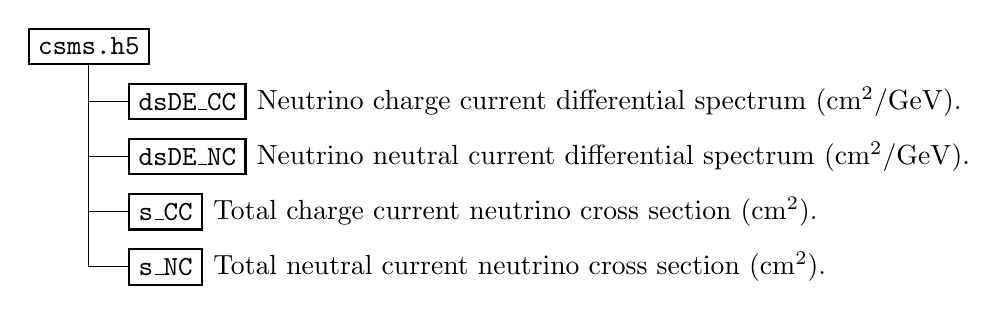
\begin{tikzpicture}[%
    grow via three points={one child at (0.5,-0.7) and
      two children at (0.5,-0.7) and (0.5,-1.4)},
    edge from parent path={(\tikzparentnode.south) |- (\tikzchildnode.west)}]
    \node {{\ttf csms.h5}}
    child { node [label=right:{Neutrino charge current differential spectrum (${\rm cm^2/GeV}$).}]  {\ttf dsDE\_CC}}
    child { node [label=right:{Neutrino neutral current differential spectrum (${\rm cm^2/GeV}$).}] {\ttf dsDE\_NC}}
    child { node [label=right:{Total charge current neutrino cross section (${\rm cm^2}$).}]{\ttf s\_CC}}
    child { node [label=right:{Total neutral current neutrino cross section (${\rm cm^2}$).}] {\ttf s\_NC}}
    ;
  \end{tikzpicture}
  \caption{HDF5 cross section format.}
  \label{fig:nusquids_cross_section_hdf5}
\end{figure}


\subsubsection{Constructors}

\begin{itemize}
\item Default constructor.
  \begin{lstlisting}
    NeutrinoDISCrossSectionsFromTables();
  \end{lstlisting}
  This constructor load the defaults {\ttf csms.h5} file
\end{itemize}

The files to load the different cross-sections can be specified
explicitly as follows. 
\begin{lstlisting}
  NeutrinoDISCrossSectionsFromTables csh5('./csms.h5');
  NeutrinoDISCrossSectionsFromTables cstxt('./nusigma_');
\end{lstlisting}

\subsubsection{Functions}

\begin{itemize}
\item Total cross sections
  \begin{lstlisting}
    double TotalCrossSection(double Enu,
    	NeutrinoFlavor flavor, NeutrinoType neutype,
    	Current current) const;
      \end{lstlisting}
      
  Returns the total cross section at an energy {\ttf Enu} in eV, neutrino
  flavor {\ttf flavor}, neutrino type: {\ttf neutype}, and {\ttf
    current} can be either {\ttf NC} or {\ttf CC} for neutral or
  charge current DIS cross sections. Using a linear interpolation in
  the logarithm of the neutrino energy. 
     
\item Single differential cross sections              
  \begin{lstlisting}
    double SingleDifferentialCrossSection(double E1, double E2,
    	NeutrinoFlavor flavor, NeutrinoType neutype,
    	Current current) const;
  \end{lstlisting}
      Function that given an incident neutrino energy ({\ttf E1}) in eV an outgoing lepton energy ({\ttf E2}), as well as neutrino flavor,
       type, and process, returns the differential cross section with
       respect to the outgoing lepton energy in ${\rm cm}^2/{\rm
         GeV}$. Using a bi-linear interpolation. 
\end{itemize}

\subsubsection{GlashowResonanceCrossSection}

This class implements the formulas in~\citep{GhandiReno} in order to calculate the electron antineutrino Glashow resonance cross section contribution.

\subsubsection{Constructors}

\begin{itemize}
\item Default constructor.
  \begin{lstlisting}
    GlashowResonanceCrossSection();
  \end{lstlisting}
\end{itemize}

\subsubsection{Functions}

\begin{itemize}
\item Total cross sections
  \begin{lstlisting}
    double TotalCrossSection(double Enu,
    	NeutrinoFlavor flavor, NeutrinoType neutype,
    	Current current) const;
  \end{lstlisting}
     Returns the total cross section in cm$^2$ at an energy {\ttf Enu} in eV, neutrino flavor {\ttf flavor}, and neutrino type: {\ttf neutype}.
     If the flavor is not electron and neutrino type is not antineutrino it returns zero.              
\item Single differential cross sections
  \begin{lstlisting}
    double SingleDifferentialCrossSection(double E1, double E2,
    	NeutrinoFlavor flavor, NeutrinoType neutype,
    	Current current) const;
  \end{lstlisting}
  Returns the single differential cross section in cm$^2$/GeV for an incident neutrinos energy ({\ttf
    E1}) in eV an outgoing neutrinos energy ({\ttf E2}) in eV, neutrino flavor ({\ttf flavor}), 
  and neutrino type ({\ttf neutype}).
     If the flavor is not electron and neutrino type is not antineutrino it returns zero.   
      
\end{itemize}

\subsection{TauDecaySpectra}

This object can be query to obtain $\tau$ decay physics into leptons
and hadrons. The formulas implemented in this class were taken
from~\citep{Dutta:2000jv}. It is only used when $\tau$-regeneration is
activated and it returns the following quantities on the energy
nodes, 
\begin{equation}
\frac{dN^{lep/had}_{dec} (E_\tau, E_\nu)}{dE_\nu} {\rm ~~and~~ }
\frac{d\bar{N}^{lep/had}_{dec} (E_\tau, E_\nu)}{dE_\nu},
\label{eqn:tau-dist}
\end{equation}
i.e. the neutrino and antineutrino spectral distributions from $\tau$
leptonic and hadronic decay modes. 

\subsubsection{Constructors and Initializing Functions}

\begin{itemize}
\item Default constructor.
  \begin{lstlisting}
    TauDecaySpectra();
  \end{lstlisting}
\item Constructor and initializing function with memory reservation.
  \begin{lstlisting}
    TauDecaySpectra(marray<double,1> E_range);
    void Init(marray<double,1> E_range);
  \end{lstlisting}
This constructor and initialization functions calculate and store the
$\tau$ decay spectra on nodes specified by the one dimensional array
{\ttf E\_range} in eV.
\end{itemize}

\subsubsection{Functions}

The following functions assume that the $\tau$ and $\bar{\tau}$ have
the same decay distribution. 

\begin{itemize}
\item (Anti)Neutrino spectra with respect to neutrino energy.
  \begin{lstlisting}
    double dNdEnu_All(int e1,int e2) const;
  \end{lstlisting}
  Returns neutrino decay spectra evaluated from energy node
  {\ttfamily e1} to energy node {\ttfamily e2} when $\tau$ decays into
  leptons or hadrons.  
  \begin{lstlisting}
    double dNdEnu_Lep(int e1,int e2) const;
  \end{lstlisting}
  Returns neutrino decay spectra evaluated between energy nodes
  {\ttfamily e1} and {\ttfamily e2} when $\tau$ decays into leptons. 
\item (Anti)Neutrino spectra with respect to $\tau$ energy.
  \begin{lstlisting}
    double dNdEle_All(int e1,int e2) const;
  \end{lstlisting}
  Returns neutrino decay spectra evaluated between energy nodes
  {\ttfamily e1} and {\ttfamily e2} when $\tau$ decays into leptons
  or hadrons with respect to the initial $\tau$ energy.
  \begin{lstlisting}
    double dNdEle_Lep(int e1,int e2) const;
  \end{lstlisting}
  Returns neutrino decay spectra evaluated between energy nodes
  {\ttfamily e1} and {\ttfamily e2} when $\tau$ decays into
  leptons with respect to the initial $\tau$ energy.
\item Get the $\tau$ branching ratio to leptons.
  \begin{lstlisting}
    double GetTauToLeptonBranchingRatio() const;
  \end{lstlisting}
  Returns the $\tau$ branching ratio to leptons.
\item Get the $\tau$ branching ratio to hadrons.
  \begin{lstlisting}
    double GetTauToHadronBranchingRatio() const;
  \end{lstlisting}
  Returns the $\tau$ branching ratio to hadrons.
\end{itemize}

\subsection{nuSQUIDS}

This object is an specialization of the {\ttf SQUIDS} class~\citep{SQUIDS} that implements the
differential equations as described in Sec.~\ref{sec:theory}. In
particular, it is used to specify the propagation {\ttf Body} and its
associated {\ttf Track}. Moreover, it uses the {\ttf
  NeutrinoCrossSections} and {\ttf TauDecaySpectra} in order to
evaluate the neutrino cross sections and $\tau$ decay spectra; the
latter is only used then {\it $\tau$} regeneration is
enabled. Furthermore, it enables the user to modify the neutrino
oscillation parameters as well as the differential equation numerical
precision. Finally, it also has the capability to create and read HDF5
files that store the program results and configuration. 

\subsubsection{Constructors}

\begin{itemize}
\item Default constructor.
  \begin{lstlisting}
    nuSQUIDS();
  \end{lstlisting}
\item Move constructor.
  \begin{lstlisting}
    nuSQUIDS(nuSQUIDS&&);
  \end{lstlisting}
Constructs a {\ttf nuSQUIDS} object from an r-value reference.  
\item Single energy mode constructor.
  \begin{lstlisting}
    nuSQUIDS(unsigned int numneu, NeutrinoType NT);
  \end{lstlisting}
This constructor and initialization function initializes {\ttfamily nuSQUIDS} in the
single energy mode. {\ttfamily numneu} specifies the number of
neutrino flavors which can go from two to six, while {\ttfamily NT} can be
set to  {\ttfamily neutrino} or {\ttfamily antineutrino}. 
\item Multiple energy mode constructor.
  \begin{lstlisting}
    nuSQUIDS(marray<double,1> E_vector,
    unsigned int numneu,NeutrinoType NT = both,
    bool iinteraction = false,
    std::shared_ptr<NeutrinoCrossSections> ncs = nullptr)
  \end{lstlisting}
This constructor and initialization function initializes {\ttfamily nuSQUIDS} in the
multiple energy mode. We need to provide the following arguments:
list of neutrino energy nodes
(\lstinline[columns=fixed,breaklines=true]{E_vector}),
number of neutrino flavors ({\ttf numneu}), neutrino or
anti-neutrino type ({\ttf NT}),  non-coherent scattering
interactions ({\ttf iinteraction}), and neutrino cross section object
pointer ({\ttf ncs}).  

\item Constructing from a $\nu$SQuIDS-HDF5 file
  \begin{lstlisting}
    nuSQUIDS(std::string hdf5_filename, std::string grp = "/",
    std::shared_ptr<InteractionStructure> int_struct = nullptr)
  \end{lstlisting}
This constructor initializes {\ttfamily nuSQUIDS} from a 
previously generated $\nu$SQuIDS HDF5 file. {\ttfamily filepath} must
specify the full path of the HDF5 file, {\ttfamily grp} specifies the
location on the HDF5 file structure where the object will be saved (by default
it will be saved on the {\ttfamily root} of the HDF5 file), and {\ttf
  int\_struct} can specify the cross-section object instead of loading it from
the file.
\end{itemize}

\subsubsection{Functions}

\textbf{Functions to evaluate flavor and mass composition}

\begin{itemize}
\item Flavor composition evaluator (single energy mode)
  \begin{lstlisting}
    double EvalFlavor(unsigned int flv) const;
  \end{lstlisting}
Returns the content a given neutrino flavor specified by {\ttfamily
  flv} ({\ttfamily 0 = $e$}, {\ttfamily 1 = $\mu$}, {\ttfamily 2 =
  $\tau$}, ...). This function can only be use in the single energy
mode. 
\item Flavor composition evaluator (multiple energy mode)
  \begin{lstlisting}
    double EvalFlavorAtNode(unsigned int flv, unsigned int ie, 
                            unsigned int rho=0) const;
    double EvalFlavor(unsigned int flv, double enu,
                      unsigned int rho=0) const;
    double EvalFlavor(unsigned int flv,double enu,
                      unsigned int rho,double scale,
                      std::vector<bool>& avr) const;
  \end{lstlisting}
{\ttfamily EvalFlavorAtNode} returns the content a given neutrino
flavor specified by {\ttfamily flv} ({\ttfamily 0 = $e$}, {\ttfamily 1
  = $\mu$}, {\ttfamily 2 = $\tau$, ...}) at an energy node {\ttfamily
  ie}. Furthermore, {\ttfamily EvalFlavor} returns the approximate
content of a given flavor for a specific neutrino energy  {\ttf enu}
by interpolating in the interaction basis. In each function, when
considering  {\ttf  NT = both}, the parameter {\ttf rho} toggles
between {\ttf neutrino (0)} and {\ttf antineutrino (1)}.
The last function gets two additional arguments: an {\ttf scale} such
that all $H_0$ induced oscillation frequencies larger than this scale
will be averaged and a vector of booleans which entries will be set to
true if the corresponding oscillations frequencies have been averaged
out.


\item Mass composition evaluator (single energy mode)
  \begin{lstlisting}
    double EvalMass(unsigned int eig) const;
  \end{lstlisting}
Returns the content a given neutrino mass eigenstate specified by {\ttfamily eig} ({\ttfamily 0 = $\nu_1$}, {\ttfamily 1 = $\nu_2$}, {\ttfamily 2 = $\nu_3$, ...}). This function can only be use in the  single energy mode.
\item Mass composition evaluator (multiple energy mode)
  \begin{lstlisting}
    double EvalMassAtNode(unsigned int eig, unsigned int ie,
                           unsigned int rho=0) const;
    double EvalMass(unsigned int eig, double enu,
                     unsigned int rho=0) const;
    double EvalMass(unsigned int flv,double enu,
                    unsigned int rho,double scale,
                    std::vector<bool>& avr) const;
  \end{lstlisting}
{\ttfamily EvalMassAtNode} returns the content a given neutrino mass
eigenstate specified by {\ttfamily eig} ({\ttfamily 0 = $\nu_1$},
{\ttfamily 1 = $\nu_2$}, {\ttfamily 2 = $\nu_3$, ...}) at an energy
node {\ttfamily ie}. Furthermore, {\ttfamily EvalMass} returns the
approximate content of a given mass eigenstate for a specific neutrino
energy  {\ttf enu} by interpolating in the interaction basis. In each
function, when considering  {\ttf  NT = both}, the parameter {\ttf
  rho} toggles between {\ttf neutrino (0)} and {\ttf antineutrino
  (1)}. The last function gets two additional arguments: an {\ttf scale} such
that all $H_0$ induced oscillation frequencies larger than this scale
will be averaged and a vector of booleans which entries will be set to
true if the corresponding oscillations frequencies have been averaged
out.
\end{itemize}

\textbf{Functions to evolve the neutrino ensemble}

\begin{itemize}
\item Evolve state
  \begin{lstlisting}
    void EvolveState();
  \end{lstlisting}
Once the neutrino propagation problem has been setup this function
evolves the neutrino state from its initial position to its final
position specified by the {\ttfamily track}. 
\end{itemize}

\textbf{Functions obtain properties of the nuSQUIDS object as well as the state}

\begin{itemize}
\item Get energy nodes values
  \begin{lstlisting}
    marray<double,1> GetERange() const;
  \end{lstlisting}
  Returns a one dimensional array containing the energy nodes
  positions given in eV. 
  \item Get number of energy nodes
  \begin{lstlisting}
    unsigned int GetNumE() const;
  \end{lstlisting}
  Returns the number of energy nodes.
  \item Get number neutrino flavors
  \begin{lstlisting}
    unsigned int GetNumNeu() const;
  \end{lstlisting}
  Returns the number of neutrino flavors.
  \item Get Hamiltonian at current position
  \begin{lstlisting}
    SU_vector GetHamiltonian(unsigned int ie, 
                             unsigned int rho = 0);
  \end{lstlisting}
  Returns the {\ttf SU\_vector} that represents the (anti)neutrino
  Hamiltonian at the current position, at a given energy node {\ttf
    ie}, and  {\ttf rho} specifies whether the neutrino or antineutrino.
  \item Get the state of the system 
  \begin{lstlisting}
    const squids::SU_vector& GetState(unsigned int ei,
        unsigned int rho = 0) const;
  \end{lstlisting}
  Returns the {\ttf SU\_vector} that represents the (anti)neutrino state at given energy node {\ttf ie}. 
  Furthermore, {\tt rho} specifies whether the neutrino or antineutrino state is returned.
  \item Get the flavor projector
  \begin{lstlisting}
    SU_vector GetFlavorProj(unsigned int ie,
         unsigned int rho = 0) const;
  \end{lstlisting}
  Returns a {\ttf SU\_vector} that represents the flavor projector for the energy node {\ttf ie} and 
  {\ttf rho} specifies if neutrinos or antineutrinos are requested.
  \item Get the mass projector
  \begin{lstlisting}
    SU_vector GetMassProj(unsigned int ie,
         unsigned int rho = 0) const;
  \end{lstlisting}
  Returns a {\ttf SU\_vector} that represents the mass projector for the energy node {\ttf ie} and 
  {\ttf rho} specifies if neutrinos or antineutrinos are requested.
  \item Get {\ttfamily Body}
  \begin{lstlisting}
    std::shared_ptr<Body> GetBody() const;
  \end{lstlisting}
  Returns the {\ttf Body} instance currently stored in the {\ttf nuSQUIDS} object.
  \item Get {\ttfamily Track}
  \begin{lstlisting}
    std::shared_ptr<Track> GetTrack() const;
  \end{lstlisting}
  Returns the {\ttf Track} instance currently stored in the {\ttf nuSQUIDS} object.
  \item Get mixing angle
  \begin{lstlisting}
    double Get_MixingAngle(unsigned int i, unsigned int j) const;
  \end{lstlisting}
  Returns the $\theta_{i,j}$ mixing angle where {\ttf i} and {\ttf j} are zero based indexes.
  \item Get CP phase
  \begin{lstlisting}
    double Get_CPPhase(unsigned int i, unsigned int j) const;
  \end{lstlisting}
  Returns the $\delta_{i,j}$ CP phase where {\ttf i} and {\ttf j} are zero based indexes.
  \item Get square mass difference
  \begin{lstlisting}
    double Get_SquareMassDifference(unsigned int i) const;
  \end{lstlisting}
  Returns the $\Delta m^2_{i0}$ in ${\rm eV}^2$ where $1\le i < {\rm \tt numneu}$.
  \end{itemize}
  
\textbf{Functions to set properties of the nuSQUIDS object as well as the state}

\begin{itemize}
  \item Set {\ttfamily Body}
  \begin{lstlisting}
    void Set_Body(std::shared_ptr<Body>);
  \end{lstlisting}
  Sets the {\ttf Body} instance in which the neutrino propagation will take place.
  \item Set {\ttfamily Track}
  \begin{lstlisting}
    void Set_Track(std::shared_ptr<Track>);
  \end{lstlisting}
  Sets the {\ttf Track} instance which describes the neutrino propagation inside a
  given {\ttf Body}.
  \item Set the initial state
  \begin{lstlisting}
    void Set_initial_state(marray<double,1> state, Basis basis);
    void Set_initial_state(marray<double,2> state, Basis basis);
    void Set_initial_state(marray<double,3> state, Basis basis);
  \end{lstlisting}
  {\ttf Set\_initial\_state} sets the initial neutrino (and
  antineutrino) state. The states  can be specified for the single and
  multiple energy modes can be specified using the different {\ttf
    C++} signatures. In each case {\ttf basis} can be either {\ttf
    mass} or {\ttf flavor}. 
  \begin{itemize}
  	\item {\ttf marray<double,1> state}: 
	Can only be used in single energy mode and is defined by 
	{\ttf state[$\alpha$]  = $\phi_\alpha$ } where $\alpha$ is a
        flavor or mass eigenstate index. 
	\item {\ttf marray<double,2> state}: Can only be used in
          multiple energy mode and is defined by {\ttf
            state[ei][$\alpha$]  = $\phi_\alpha (E$[ei]$),$ } i.e. the
          flavor (mass) eigenstate composition at a given energy node
          {\ttf ei}. 
	\item {\ttf marray<double,3> state}: Can only be used in
          multiple energy mode and is defined by {\ttf
            state[ei][$\rho$][$\alpha$]  = $\phi^{\rho}_\alpha
            (E$[ei]$),$ } i.e. the flavor (mass) eigenstate
          composition at a given energy node {\ttf ei}, and where
          $\rho = 0 \equiv {\rm neutrino}$ and $\rho = 0 \equiv {\rm
            antineutrino}$. 
  \end{itemize}
  \item Set energy
  \begin{lstlisting}
    void Set_E(double enu);
  \end{lstlisting}
  Set the neutrino energy. This function can only be used in the
  single energy mode and {\ttf enu} has to be in natural units.
  \item Enable progress bar
  \begin{lstlisting}
    void Set_ProgressBar(bool opt);
  \end{lstlisting}
  If {\ttf opt} is {\ttf true} a progress bar will be printed to
  indicate the calculation progress. 
  \item Enable tau regeneration
  \begin{lstlisting}
    void Set_TauRegeneration(bool opt);
  \end{lstlisting}
  If {\ttf opt} is {\ttf true}, {\ttf NT} is {\ttf both}, and non
  coherent interactions are enabled tau regeneration effects will be included.
  \item Set mixing angle
  \begin{lstlisting}
    void Set_MixingAngle(unsigned int i, unsigned int j,
        double angle);
  \end{lstlisting}
  Sets the $\theta_{i,j}$ mixing angle to {\ttf angle}, where {\ttf i}
  and {\ttf j} are zero based indexes, and {\ttf angle} must be given in radians.
  \item Get CP phase
  \begin{lstlisting}
    void Set_CPPhase(unsigned int i, unsigned int j,
        double phase);
  \end{lstlisting}
  Sets the $\delta_{i,j}$ CP phase to {\ttf phase}, where {\ttf i} and
  {\ttf j} are zero based indexes, and {\ttf phase} must be given in radians.
  \item Set square mass difference
  \begin{lstlisting}
    void Set_SquareMassDifference(unsigned int i, doble dmsq);
  \end{lstlisting}
  Sets the $\Delta m^2_{i0}$ to {\ttf dams}, given in ${\rm eV}^2$,
  where $1\le i < {\rm \tt numneu}$. 
  \item Set parameters to default
  \begin{lstlisting}
    void Set_MixingParametersToDefault();
  \end{lstlisting}
  Sets the mixing angles and square mass mixings to the best fit point
  given in \citep{Gonzalez-Garcia:2014bfa}. 
  \item Set the basis of solution
  \begin{lstlisting}
    void Set_Basis(Basis basis);
  \end{lstlisting}
  Sets the basis on which the evolution will be performed. Two options
  are available: {\ttf mass} and {\ttf interaction}, the later being
  the default. 
\item Set neutrino cross-section
  \begin{lstlisting}
    void SetNeutrinoCrossSections(
        std::shared_ptr<NeutrinoCrossSections> xs)
  \end{lstlisting}
  Sets the neutrino cross-section~\ref{sec:xs} given by the shared
  pointer {\ttf xs} to the nuSQuIDS object.
\end{itemize}
  
\textbf{HDF5 interface functions}
 
\begin{itemize}
  \item Write nuSQUIDS object into an HDF5 file.
  \begin{lstlisting}
    void WriteStateHDF5(std::string hdf5_filename,
                        std::string group = "/",
                        bool save_cross_sections = true, 
                        std::string cross_section_grp_loc = "")
                        const;
  \end{lstlisting}
  Writes the current {\ttf nuSQUIDS} configuration and state into an HDF5 file
  for later use. {\ttf hdf5\_filename} specifies the output filename, {\ttf group} is the 
  location on the HDF5 structure where the {\ttf nuSQUIDS} object will be save; by default
  the root of the HDF5 will be used. Furthermore, {\ttf
    save\_cross\_sections} and {\ttf cross\_section\_grp\_loc} specify
  if cross sections will be saved and where on the HDF5 file
  structure. See Figure~\ref{fig:nusquids_hdf5}. 
  \item Add to the HDF5 write funtion.
  \begin{lstlisting}
    virtual void AddToWriteStateHDF5(hid_t hdf5_loc_id) const;
  \end{lstlisting}
  En ables the user to add content in the HDF5 file. An HDF5
  location,{\ttf hdf5\_loc\_id}. Using that the user can stor relevant
  informa about the derived nuSQuIDS class.
  \item Read nuSQUIDS object from an HDF5 file.
    \begin{lstlisting}
    void ReadStateHDF5(std::string hdf5_filename,
                       std::string group = "/",
                       std::string cross_section_grp_loc = "");
  \end{lstlisting}
  Reads an previously generated HDF5 file and sets the {\ttf nuSQUIDS} object
  accordingly, i.e. it configures it and loads the saved state. {\ttf
    hdf5\_filename} specifies the input filename, {\ttf group} is the
  location on the HDF5 structure where the {\ttf nuSQUIDS} object is;
  by default the root of the HDF5 is assumed. Furthermore, {\ttf
    cross\_section\_grp\_loc} specify where the cross sections are in
  the HDF5 file structure. See Figure~\ref{fig:nusquids_hdf5}. 
  \item Add to the HDF5 read file.
  \begin{lstlisting}
    virtual void AddToReadStateHDF5(hid_t hdf5_loc_id);
  \end{lstlisting}
  Enables the user to read user defined content from the HDF5 file. An
  HDF5 location,{\ttf hdf5\_loc\_id}, is provided so the user can
  interface with the HDF5 library. For a correct implementations this
  functions has to be implemented consistently with {\ttf
    AddToWriteStateHDF5} function. 
\end{itemize}

\begin{figure}[htb]
\centering
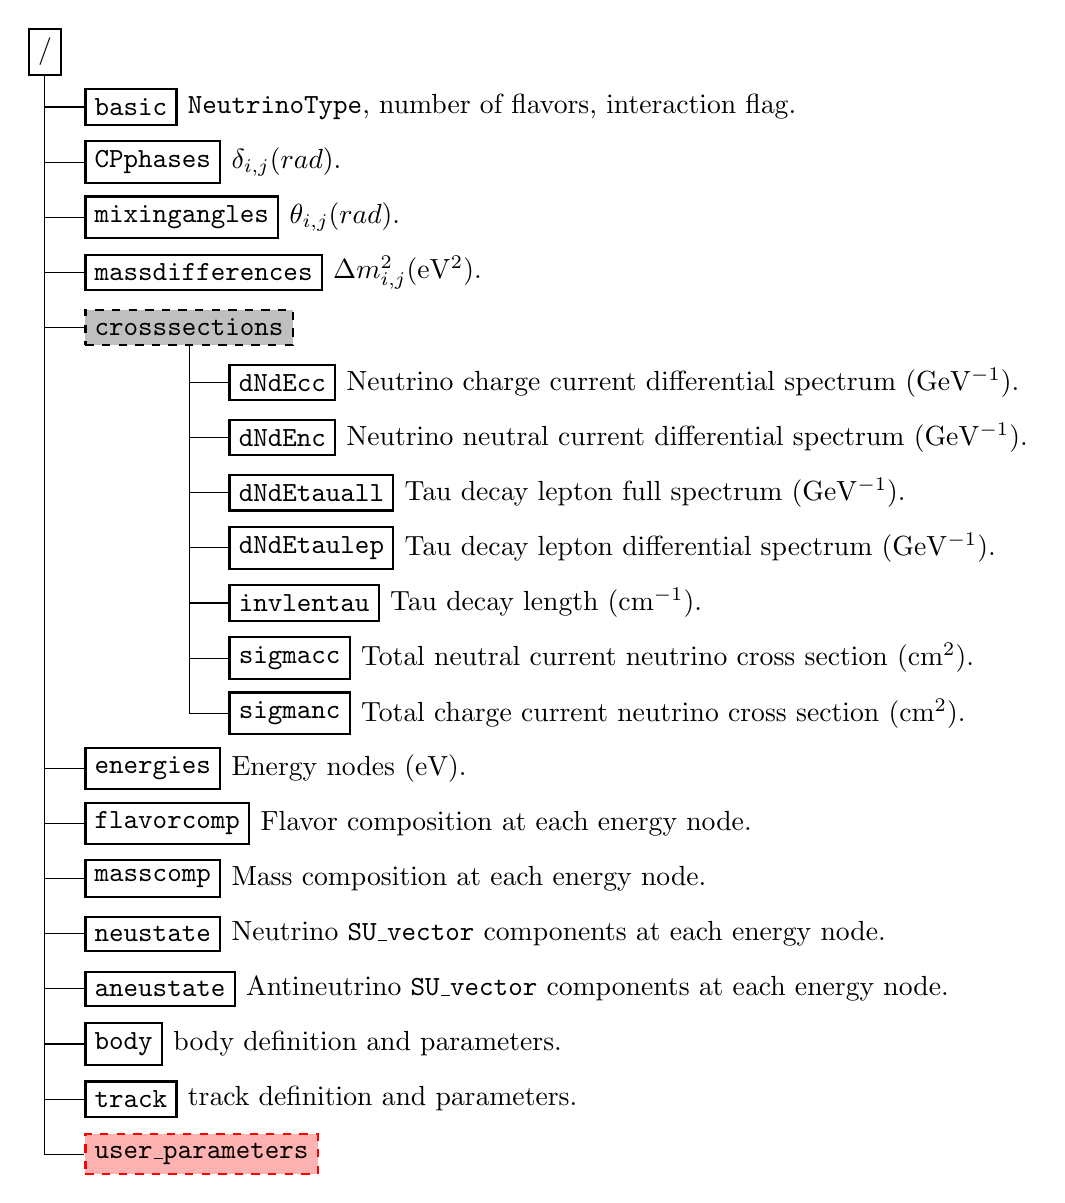
\begin{tikzpicture}[%
  grow via three points={one child at (0.5,-0.7) and
  two children at (0.5,-0.7) and (0.5,-1.4)},
  edge from parent path={(\tikzparentnode.south) |- (\tikzchildnode.west)}]
  \node {/}
    child { node [label=right:{{\ttf NeutrinoType}, number of flavors, interaction flag.}] {\ttf basic}}	
    child { node [label=right:{$\delta_{i,j} (rad).$}] {\ttf CPphases}}		
    child { node [label=right:{$\theta_{i,j} (rad).$}] {\ttf mixingangles}}
    child { node [label=right:{$\Delta m^2_{i,j} (\rm eV^2).$}] {\ttf massdifferences}}
    child { node [optional] {\ttf crosssections}
      child { node [label=right:{Neutrino charge current differential spectrum (${\rm GeV^{-1}}$).}]  {\ttf dNdEcc}}
      child { node [label=right:{Neutrino neutral current differential spectrum (${\rm GeV^{-1}}$).}] {\ttf dNdEnc}}
      child { node [label=right:{Tau decay lepton full spectrum (${\rm GeV^{-1}}$).}] {\ttf dNdEtauall}}
      child { node [label=right:{Tau decay lepton differential spectrum (${\rm GeV^{-1}}$).}] {\ttf dNdEtaulep}}
      child { node [label=right:{Tau decay length (${\rm cm^{-1}}$).}] {\ttf invlentau}}
      child { node [label=right:{Total neutral current neutrino cross section (${\rm cm^2}$).}]{\ttf sigmacc}}
      child { node [label=right:{Total charge current neutrino cross section (${\rm cm^2}$).}] {\ttf sigmanc}}
    }
    child [missing] {}				
    child [missing] {}				
    child [missing] {}
    child [missing] {}
    child [missing] {}			
    child [missing] {}
    child [missing] {}			
    child { node [label=right:{Energy nodes ({\rm eV}).}] {\ttf energies}}	
    child { node [label=right:{Flavor composition at each energy node.}] {\ttf flavorcomp}}
    child { node [label=right:{Mass composition at each energy node.}] {\ttf masscomp}}
    child { node [label=right:{Neutrino {\ttf SU\_vector} components at each energy node.}] {\ttf neustate}}
    child { node [label=right:{Antineutrino {\ttf SU\_vector} components at each energy node.}] {\ttf aneustate}}
    child { node [label=right:{body definition and parameters.}] {\ttf body}}
    child { node [label=right:{track definition and parameters.}] {\ttf track}}
    child { node [selected] {\ttf user\_parameters}}
    ;
\end{tikzpicture}
\caption{Structure of {\ttf nuSQUIDS} HDF5 file. The {\ttf
    crosssections} group will only be written when interactions are
  enable. Furthermore, {\ttf user\_parameters} are by default empty
  and can be set/access by {\ttf AddToWriteStateHDF5/AddToReadStateHDF5}.} 
\label{fig:nusquids_hdf5}
\end{figure}



\subsection{nuSQUIDSAtm}

Atmospheric neutrino oscillations is a major and instrumental part of
research in contemporary neutrino physics. Experiments like
SuperKamiokande, IceCube, and Antares have used atmospheric neutrinos
to measure neutrino mass splittings and mixing angles. Furthermore,
proposed extensions like HyperKamiokande, PINGU, and ORCA ought to
improve the current measurements and have sensitivity to neutrino
neutrino mass ordering. This class allows to propagate a set of full
energy spectrum of neutrinos for a different zenith angles.
It implements functions to set easily the initial conditions and also
interpolations to the fluxes.
\subsubsection{Constructors}

\begin{itemize}
\item Constructor with {\ttf costh} range.
  \begin{lstlisting}
    template<typename... ArgTypes> nuSQUIDSAtm(
        marray<double,1> costh_array, ArgTypes&&... args)
  \end{lstlisting}
This constructor it creates a set {\ttf nuSQUIDS} or derived {\ttf
  nuSQUIDS} objects with a set of zenith angles given by the {\ttf
  marray} {\ttf costh\_array}. The arguments given in {\ttf arg} are the
corresponding arguments of the nuSQUIDS or derived nuSQUIDS class constructor.

\item Constructing from a nuSQuIDSAtm-HDF5 file
  \begin{lstlisting}
    nuSQUIDSAtm(std::string hdf5_filename)
  \end{lstlisting}
This constructor initializes {\ttfamily nuSQUIDS} from a 
previously generated $\nu$SQuIDS-HDF5 file. The result {\ttfamily nuSQUIDS} 
object will be given in {\it single} or {\it multiple} energy mode
depending on the HDF5 file configuration. {\ttfamily filepath} must specify the full
path of the HDF5 file. Furthermore,
{\ttfamily grp} specifies the location on the HDF5 file structure
where the object will be saved; by default
it will be saved on the {\ttfamily root} of the HDF5 file.

\item Move constructor.
  \begin{lstlisting}
    nuSQUIDSAtm(nuSQUIDSAtm&&);
  \end{lstlisting}

  \subsubsection{Functions}
\item Set initial state.
  \begin{lstlisting}
    void Set_initial_state(const marray<double,3>& ini_flux,
        Basis basis=flavor);
    void Set_initial_state(const marray<double,4>& ini_flux,
        Basis basis=flavor);
  \end{lstlisting}
  Sets the initial state of the system given in the marray {\ttf
    ini\_flux}, {\ttf basis} is the basis in where the state is
  defined. Different {\ttf marray} can be used for different cases:

  \begin{itemize}
  \item {\ttf marray<double,3> state}: Can only be used in
    multiple energy mode and is defined by {\ttf
      state[czi][ei][$\alpha$]  = $\phi_\alpha (E$[ei]$,costh$[czi]$),$ } i.e. the
    flavor (mass) eigenstate composition at a given energy and cosine
    zenith node {\ttf ei} and {\ttf czi}. 
  \item {\ttf marray<double,4> state}: Can only be used in
    multiple energy mode and is defined by {\ttf
      state[czi][ei][$\rho$][$\alpha$]  = $\phi^{\rho}_\alpha
      (E$[ei]$,costh$[czi]$),$ } i.e. the flavor (mass) eigenstate
    composition at a given energy and zenith node {\ttf ei} and {\ttf czi}, and where
    $\rho = 0 \equiv {\rm neutrino}$ and $\rho = 0 \equiv {\rm
      antineutrino}$. 
  \end{itemize}
  
\item Evolve function
  \begin{lstlisting}
    void EvolveState();
  \end{lstlisting}
  Function that evolves the system.

\item Evaluate the flux for a given flavor.
  \begin{lstlisting}
    double EvalFlavor(unsigned int flv,double costh,
        double enu, unsigned int rho,
        double scale,std::vector<bool> avr) const;

    double EvalFlavor(unsigned int flv,double costh,
    double enu,unsigned int rho = 0,
        bool randomize_production_height = false) const;
  \end{lstlisting}
  It returns the flux for the flavor {\ttf flv} at the value of cosine
  zenith given by {\ttf costh} and energy given by {\ttf enu}.
  {\ttf rho} is {\ttf neutrino} or {\ttf antineutrino}.
  Some arguments can be also set: If a frequency is higher that {\ttf
    scale} it will be averaged out, and the corresponding entrance in the
  Boolean vector {\ttf avr} will be set to {\ttf true}.
  In the second case the randomization on the production height of the
  neutrino can be set to $true$, by default is $false$.
  
\item Read and write function.
  \begin{lstlisting}
    void ReadStateHDF5(std::string hdf5_filename);
    void WriteStateHDF5(std::string hdf5_filename,
        bool overwrite = true) const;
  \end{lstlisting}
  
  This functions read and write the state of the system in the file
  {\ttf hdf5\_filename}, in the write {\ttf overwrite} may be set to
  {\ttf true} or {\ttf false}.

\item Set functions as in nuSQUIDS.
  \begin{lstlisting}
    void Set_MixingParametersToDefault();
    void Set_MixingAngle(unsigned int i,
                         unsigned int j,double angle);
    void Set_CPPhase(unsigned int i,
                     unsigned int j,double angle);
    void Set_SquareMassDifference(unsigned int i,double sq);
    void Set_h(double h);
    void Set_h_max(double h);
    void Set_h_min(double h);
    void Set_abs_error(double eps);
    void Set_rel_error(double eps);
    void Set_GSL_step(gsl_odeiv2_step_type const * opt);
    void Set_ProgressBar(bool opt);
    void Set_TauRegeneration(bool opt);
    void Set_GlashowResonance(bool opt);
    void Set_IncludeOscillations(bool opt);
    void Set_AllowConstantDensityOscillationOnlyEvolution(bool opt);
    void Set_PositivityConstrain(bool opt);
    void Set_PositivityConstrainStep(double step);
    void SetNeutrinoCrossSections(
                   std::shared_ptr<NeutrinoCrossSections> xs);
  \end{lstlisting}
  All this functions do a recursive call to the function with
  the same name in all the nuSQUIDS objects.
  

\item Set earth model.
  \begin{lstlisting}
    void Set_EarthModel(std::shared_ptr<EarthAtm> earth);
  \end{lstlisting}
  Sets the body given by {\ttf earth} to all the nuSQUIDS objects in
  every node.

\item Sets the number of threads
  \begin{lstlisting}
    void Set_EvalThreads(unsigned int nThreads);
  \end{lstlisting}
  The evolution can be done in a multi-thread with the number of
  threads specified by {\ttf nThreads}.

\item Set absolute error in a give node.
  \begin{lstlisting}
    void Set_abs_error(double eps, unsigned int idx);
  \end{lstlisting}
  Sets the GSL absolute error {\ttf eps} in the cosine zenith node
  given by $idx$.

\item Number of threads.
  \begin{lstlisting}
    unsigned int Get_EvalThreads() const{
  \end{lstlisting}
  Returns the number of threads used in the evaluation.
\item Get mixing angles.
  \begin{lstlisting}
    double Get_MixingAngle(unsigned int i, unsigned int j) const;
  \end{lstlisting}
  It returns the mixing angle of the first cosine zenith node in the
  rotation plane given by ({\ttf i}, {\ttf j}).

\item Get square mass difference.
  \begin{lstlisting}
    double Get_SquareMassDifference(unsigned int i) const;
  \end{lstlisting}
  It returns the square mass difference value given by {\ttf i}.
 \item Number of energy nodes.
  \begin{lstlisting}
    size_t GetNumE() const;
  \end{lstlisting}
  Gives the number of energy nodes.

 \item Number of cosine zenith nodes.
  \begin{lstlisting}
    size_t GetNumCos() const;
  \end{lstlisting}
  Gives the number of cosine zenith nodes.

\item Number of rho.
  \begin{lstlisting}
    unsigned int GetNumRho() const;
  \end{lstlisting}
  Gives the number of {\ttf rho}, for neutrino-antineutrino case it
  will be two. 

\item  Energy array. 
  \begin{lstlisting}
    marray<double,1> GetERange() const;
  \end{lstlisting}
  Returns and {\ttf marray} with the value of the energies in the
  energy nodes.

\item Cosine zenith array.
  \begin{lstlisting}
    marray<double,1> GetCosthRange() const;
  \end{lstlisting}
  Returns and {\ttf marray} with the value of the cosine zenith in the
  cosine zenith nodes.

\item Get the nuSQUIDS object.
  \begin{lstlisting}
    BaseSQUIDS& GetnuSQuIDS(unsigned int ci);
  \end{lstlisting}
  Returns the nuSQUIDS object in the cosine zenith node {\ttf ci}.

\item Get the array of nuSQUIDS.
  \begin{lstlisting}
      std::vector<BaseSQUIDS>& GetnuSQuIDS();
    \end{lstlisting}
    Returns a {\ttf std::vector} with the nuSQUIDS objects in all the
    cosine zenith nodes.
\end{itemize}

% TODO: section describing space and time complexity, benchmarks

\section{Python Interface}

As the particle physics community has transition from {\ttfamily FORTRAN} to {\ttfamily C++} based frameworks, it is also a current trent to be able to interface analysis software with high-level interpreted languages such as {\ttfamily Mathematica}, {\ttfamily R}, and {\ttfamily Python}. Of these languages we have decided to implement bindings with Python due to the well-developed {\ttfamily C++}-{\ttfamily Python} bindings given by the {\ttfamily Boost} library.

\subsection{Installation}

In order to install nuSQuIDS python bindings additional libraries are required, namely, {\ttfamily Boost.Python} ($\ge1.54$) and {\ttfamily Python.numpy} ($\ge1.7$). Upon installing these new prerequisites you can run the following command to generate a Makefile to compile the bindings

\begin{lstlisting}[language=Bash]
./configure --with-python-bindings
\end{lstlisting}

This command will try to autodetect the location of the the aboved mentioned libraries. The following configuration script flags are influencial
\begin{itemize}
  \item Specify the Python executable
  \begin{lstlisting}
    --python-bin=PYTHON_EXECUTABLE
  \end{lstlisting}
  The provided {\ttf Python} executable will be use to find the python version, libraries, and includes.
  \item Set Boost library and include paths
  \begin{lstlisting}
    --with-boost=DIR
    --with-boost-incdir=DIR
    --with-boost-libdir=DIR
  \end{lstlisting}
  The {\ttf incdir} and {\ttf libdir} options are use to set the boost include and library directories. The first option is a convenient flat that sets both to directories to: {\ttf DIR/lib} and {\ttf DIR/include} for the library and include directory.

\end{itemize}
This will produce a {\ttf Makefile} in the {\ttf resource/python/src} directory of nuSQuIDS. This Makefile will be compiled when you run {\ttf make} on the main nuSQuIDS folder. This will produce a shared library in {\ttf resource/python/pybindings}; in order to be able to use the python bindings you need to add this directory to the system variable {\ttf PYTHONPATH}. {\it E.g.}, in the Bash shell
\begin{lstlisting}[language=Python]
export PYTHONPATH=NUSQUIDS_DIR/resource/python/bindings:$PYTHONPATH
\end{lstlisting}

After successful installation you can import the python bindings in the following manner
\begin{lstlisting}[language=Python]
import nuSQUIDSpy
\end{lstlisting}
where here we have introduce the alias {\ttfamily nsq} for the nuSQuIDS python module. We can further extend the
capabilities of nuSQuIDS in {\ttfamily Python} by means of the the {\ttfamily nuSQUIDSTools} module.
When it is loaded the nuSQuIDS functions and objects get overloaded with additoinal functionalities. In order to enable them, after loading the {\ttfamily nuSQUIDSpy} module, do
\begin{lstlisting}[language=Python]
import nuSQUIDSTools
\end{lstlisting}

\subsection{Description of the interface}

The interface is implemented in two files {\ttf nuSQUIDSpy.h} and {\ttf nuSQUIDSpy.cpp}. Additionally in {\ttf resources/python/inc} the file {\ttf container\_conversions.h} is provided to enable translation between {\ttf std::vector<type>} to  {\ttf List} among {\ttf C++} and {\ttf Python}. The python bindings header contains {\ttf C++} templates that facilitate registrion of {\ttf nuSQuIDS} python bindings.

In the bindings source file the following classes have been registered:
\begin{itemize}
  \item nuSQuIDS
\end{itemize}
for all these classes we have implemented the public members described on this document with the same names as on the {\ttf C++} interface.

Also, the following enumerations have been made available in {\ttf Python}
\begin{itemize}
  \item \lstinline[columns=fixed,breaklines=true]{GSL_STEP_FUNCTIONS} enumeration contains the following members: 
    \begin{itemize}
      \item \lstinline[columns=fixed,breaklines=true]{GSL_STEP_RK2},
      \item \lstinline[columns=fixed,breaklines=true]{GSL_STEP_RK4},
      \item \lstinline[columns=fixed,breaklines=true]{GSL_STEP_RKF45},
      \item \lstinline[columns=fixed,breaklines=true]{GSL_STEP_RKCK},
      \item \lstinline[columns=fixed,breaklines=true]{GSL_STEP_RK8PD},
      \item and \lstinline[columns=fixed,breaklines=true]{GSL_STEP_MSADAMS}.
    \end{itemize}
    These can be used in the {\ttf Set\_GSL\_step} \nuSQUIDS member function.
  \item {\ttf Basis}, which contains the members:
    \begin{itemize}
      \item {\ttf mass} ({\ttf Basis::mass}),
      \item {\ttf flavor} ({\ttf Basis::flavor}),
      \item and {\ttf interaction} ({\ttf Basis::interaction}).
    \end{itemize}
  \item {\ttf NeutrinoCrossSections\_NeutrinoFlavor}, which contains the members:
    \begin{itemize} 
      \item {\ttf electron} ({\ttf NeutrinoCrossSections::NeutrinoFlavor::electron}),
      \item {\ttf muon} ({\ttf NeutrinoCrossSections::NeutrinoFlavor::muon}),
      \item {\ttf tau} ({\ttf NeutrinoCrossSections::NeutrinoFlavor::tau}),
      \item and {\ttf sterile} ({\ttf NeutrinoCrossSections::NeutrinoFlavor::sterile}).
    \end{itemize}
  \item {\ttf NeutrinoCrossSections\_NeutrinoType}, which contains the members:
    \begin{itemize} 
      \item {\ttf neutrino} ({\ttf NeutrinoCrossSections::NeutrinoType::neutrino})
      \item and {\ttf antineutrino} ({\ttf NeutrinoCrossSections::NeutrinoType::antineutrino}).
    \end{itemize}
  \item {\ttf NeutrinoCrossSections\_Current}, which contains the members:
    \begin{itemize}
      \item {\ttf CC} ({\ttf NeutrinoCrossSections::Current::CC}),
      \item {\ttf NC} ({\ttf NeutrinoCrossSections::Current::NC}),
      \item and {\ttf GR} ({\ttf NeutrinoCrossSections::Current::GR}).
    \end{itemize}
  \item {\ttf Neutrinotype}, which contains the members:
    \begin{itemize}
      \item {\ttf neutrino} ({\ttf NeutrinoType::neutrino}),
      \item {\ttf antineutrino} ({\ttf NeutrinoType::antineutrino}),
      \item and {\ttf both} ({\ttf NeutrinoType::both}).
    \end{itemize}

\end{itemize}

\subsection{Examples}

\begin{lstlisting}[language=Python, frame=leftline, numbers=left, breaklines=true]
import nuSQUIDSTools
\end{lstlisting}

\subsection{Extending the interface with user-defined classes~\label{sec:python_extensions}}

In this section we briefly how to construct python bindings for user defined classes. As an example
we have an extension class called {\ttf nuSQUIDSExt} defined as:

\begin{lstlisting}[language=C++, frame=leftline, numbers=left, breaklines=true]
class nuSQUIDSExt : public nuSQUIDS {
  ...
}
\end{lstlisting}

\section{Conclusions}
\label{sec:conclu}

In this article we have written in detail the equations that guide the evolution of an ensemble of neutrinos
in a dense medium. We have described the \nuSQUIDS~ library that solves these equations. We have provide examples
of the core features of the library. We also discuss its performance and the tests that the library.
\nuSQUIDS~  provides a complete solution to the neutrino propagation when accounting for neutrino oscillations and scatterings. 
We find that it is competitive with dedicated neutrino oscillation calculators, when the number of evaluations of the oscillation probability
is large; which is the typical case of interest in neutrino experiments.
The library also has a {\ttf Python} extension which we also expose. Finally, the \nuSQUIDS~ library has been designed to be easily extendable 
onto new mediums, but onto new physics scenarios. Users contributions to the project are encourage and a number of additional
models have already been implemented and are linked in {\ttf resources/user\_contributions}.

\section*{Acknowledgements}

We thank: Jakov Van Santen for implementing the Glashow resonance cross sections;
Benjamin Jones for early adoption of this code onto the sterile analysis;
Melanie Day for early adoption of this code onto her analysis, carefully checking the non-standard interaction extension, and providing feedback;
Tianlu Yuan for comments on neutrino cross section utilities and testing the performance of the code in realistic analysis scenarios;
Subir Sarkar for providing the code to generate neutrino-nucleon the cross section tables;
Kotoyo Hoshima and Aaron Vincent for dedicated comparisons and checks of this code;
Zander Moss performing an independent check of several core features of the code;
Felix Kallenborn for carefully reading thorugh the code, writing a GPU version of the algorithm, and pointing out an improve handling of the GSL ODE solver;
Jos\'e Carpio and Zander Moss for pointing out the need to improve the Earth density interpolation;
Mauricio Bustamante for testing the Python V3 support;
Austin Schneider for reading through this draft and testing the Ubuntu support;
Tom Studdard for providing feedback and contribution of neutrino decoherence;
Jos\'e Carpio, Alberto Gago, and Eduardo Massoni for providing feedback and implemeting nuSQuIDS in GLoBES;
Zander Moss, Marjon Moulai, and Janet Conrad for providing feedback and contribution of neutrino decay extension;
Shivesh Mandalia and Teppei Katori for checking, providing feedback, and contribution on the Lorentz Violation model implementation;
Joshua Highnight and Jessie Micallef for providing a modified version of Prob3++ with NSI for detailed comparisons; and
Thomas Ehrhardt for performing detailed comparison between this code speed and accuracy versus Prob3++ CPU and GPU version.
Pedro Machado, Aaron Vincent, and Logan Wille for providing the Solar model files and useful discussion in the construction of the SolarTransition extension.
CAA is supported by U.S. National Science Foundation (NSF) grant PHY-1505858.
JS is supported by
CNW is supported by.

\bibliographystyle{plainnat}
%\bibliographystyle{apacite}
%\bibliographystyle{elsarticle-harv}

\bibliography{nusquids}

\end{document}

